\documentclass[]{phdthesis}
\usepackage{algpseudocode,algorithm,algorithmicx}
\newcommand*\Let[2]{\State #1 $\gets$ #2}
\algrenewcommand\algorithmicrequire{\textbf{Precondition:}}
\algrenewcommand\algorithmicensure{\textbf{Postcondition:}}
\def\rightarrowfill@@{\arrowfill@@\relax\relbar\rightarrow}
\addbibresource{switches_ref.bib}
\begin{document}
\title{Computational design and\\characterisation of synthetic\\ genetic switches}
\author{Miriam Leon \\ Supervisor: Chris P Barnes\\ Department of Cell and Developmental
 Biology \\ University College London}
\date{}
\maketitle

\newpage
\section{Abstract}
\setcounter{secnumdepth}{4}
\setcounter{tocdepth}{4}
\tableofcontents* 
\newpage
\listoffigures
\newpage
\listoftables
\pagestyle{plain}

%% --------------------------------------------------------------
%% CHAPTERS
%% --------------------------------------------------------------

%% Chapter-1 Introduction -------------------------------------%%
\mainmatter*
\chapter{Introduction}
\section{Contents of this thesis}


%% Chapter-2 ABC-SysBio ---------------------------------------%%
\mainmatter*
\chapter{ABC-SysBio}
\section{Introduction to Bayesian model selection}

\section{Models of the genetic toggle switch}

\section{Genetic toggle switch model selection}



%% Chapter-3 Characterising the toggle switch -----------------%%
\mainmatter*
\chapter{Characterising the toggle switch}
\section{Introduction}
In this chapter, I aim to study the genetic toggle switch experimentally.  This chapter is organised as follows: In the first section I provide an overview of the circuit used and then outline the methods used for the experiments carried out. In the subsequent section I investigate the effect that the switch has on the growth rate of the bacteria. Then I examine the concentrations of the inducers and the time needed to flip the switch. 


\section{Flow cytometry and model fitting}

Flow cytometry detects the fluorescent intensity levels in individual cells. It can also provide physical information about the size and granularity of a cell via the forward and side scattering respectively. An overview of flow cytometry is shown in Figure~\ref{fig:flow_overv}. A laser excites the fluorochrome present in the bacterial cells. The fluorochromes emit a signal that is detected by channels in the optics. The signals are then all collected and analysed. A sample typically consists single cell measurements of $10^4$-$10^5$ cells. %Typically the cell populations are separated from the noise in the experiment via expert manual gating. Advances in flow cytometry technology has increased both the number of the dimensions of the datasets and the number of samples obtained, thus promoting the development for automated methods~\autocite{Johnsson:2016fd, Chen:2015bp, ONeill:2013cs}.



\begin{figure*}[tb]
	\begin{center}
		\includegraphics[scale=0.9]{chapterABCFlow/images/flow-overview.png}
	\caption[LoF caption]{\label{fig:flow_overv}: Flow cytometry. A laser excites the fluorescent proteins present in each cell. The cytometer has up to 4 lasers, violet (V), red (R), yellow (Y) and blue (B). The detectors in the optics, FL1-4 pick up the signals. The cytometer also picks up size and granularity information via the forward scatter (FSC) and side scatter (SSC) detectors. }
	\end{center}
\end{figure*}


Flow cytometry is used in synthetic biology, among others, for BioBrick characterisation~\autocite{Kelly:2009bj}, enzyme screening~\autocite{Choi:2014gb} and industrial  bioprocesses~\autocite{Diaz:2010kw}. Flow cytometry is a powerful tool for synthetic biology as it can measure multiple parameters in single cells, and process up to 35,000 cells sec\textsuperscript{-1}~\autocite{Anonymous:2015tj}. 

A drawback of flow cytometry is that the fluorescence intensity per cell is measured rather than number of proteins. Measuring absolute numbers of protein would be ideal for model fitting, but this type of biological data cannot be directly measured~\autocite{Kelwick:2014iy}. Standardization of experimental methods in flow cytometry has aided the effort to convert relative measurements, like fluorescence intensity, to absolute measurements, like GFP cell\textsuperscript{-1} s\textsuperscript{-1}~\autocite{Kelly:2009bj, Kelwick:2014iy}. 

In this chapter, I developed ABC-Flow, a method to fit computational models to experimental flow cytometry data. ABC-Flow approaches the problem of absolute protein numbers by converting the model output of GFP cell\textsuperscript{-1} s\textsuperscript{-1} to relative fluorescence intensity. ABC-Flow is a python package that uses Bayesian statistics to fit the parameters of a given model to flow cytometry time course data. The algorithm and its usage is described in Section~\ref{sec:abcflow-meth}.

%Progress has been made in the development of computational tools for the automated analysis of flow cytometry data from the field of computational immunology~\autocite{Saeys:2016im}. These tools are used for automated gating~\autocite{Lo:2008it, Aghaeepour:2011fv, Johnsson:2016fd} as well as modelling of cellular processes over time~\autocite{Bendall:2014hs, Bagwell:2015gp}. These methods are used to track different subpopulations over time, in order to follow the underlying developmental trajectory~\autocite{Saeys:2016im} and thus cannot be applied to experiments involving uniform cell populations. 


% is necessary as flow cytometry measures the intensity of the fluorescent proteins of interest in each cell.

 %On the other hand, when simulating a model, the output is measured in number of fluorescent proteins. It is thus essential to convert the simulated signal to the same format as the data, thus convert the number of fluorescent proteins to intensity measures. 

\section{Circuit overview}

The toggle switch plasmid I used here was provided by ~\textcite{Litcofsky:2012gr}. All the switch components were contained in one plasmid, pKDL071. An overview of the plasmid is shown in Figure~\ref{fig:pKDL071map}A and the sequence given in Appendix (XXX). The circuit consists of two promoters, Ptrc2 and PLtetO-1~\autocite{Lutz:1997ti}. Ptrc2 is a constitutive promoter, repressible by LacI. PLtetO-1 is also a constitutive promoter, repressible by TetR, as shown in Figure~\ref{fig:pKDL071map}B. mCherry~\autocite{Shaner:2004vy} and \acrshort{gfp}~\autocite{SHIMOMURA:1962va} are fluorescent proteins, that were added under the control of the same promoters as the repressors, and thus reflect the levels of TetR and LacI in the system. The plasmid contains kanamycin antibiotic resistance and is high copy (ColE1 origin of replication).

This system is capable of two states, GFP high and mCherry high. When \acrshort{iptg} is added to the system, it represses the repression of TetR and mCherry and thus the cells end up in the mCherry high state. When \acrshort{atc} is added to the system, it represses the repression of LacI and GFP and thus the cells end up in the GFP high state. If no inducer is added to the system it will randomly go to the GFP high or mCherry high states.

\begin{figure*}[tb]
	\begin{center}
		\includegraphics[scale=0.55]{chapterCharacterisation/images/pKDL071_overview.png}
	\caption[LoF caption]{\label{fig:pKDL071map}: The genetic toggle switch circuit used in this chapter. (A) The plasmid map of pKDL071, the plasmid containing the genetic toggle switch used in~\textcite{Litcofsky:2012gr} (B) The interactions between each element of the circuit.}
	\end{center}
\end{figure*}
\clearpage


\section{Methods}

The toggle switch plasmid was provided by the James J Collins lab in the form of a stab culture in \textit{E. coli} K-12 MG1655.

\subsection{\textit{Escherichia coli} culturing conditions}
\label{sec:overnigh_cult}

\acrfull{lb} was made by diluting \acrshort{lb} in deionized water to a concentration of \SI{25}{\gram\per\liter} and subsequently autoclaved. \acrshort{lb} agar plates were made by adding bacteriological agar to the above solution to a concentration of \SI{45}{\milli\gram\per\milli\liter} before autoclaving. The solution was then cooled down to \SI{55}{\celsius} using a water bath. If antibiotic was required it was added to the correct concentration to the cooled solution. The solution was then aliquoted to plates and left to solidify in room temperature. The plates were stored in the fridge for up to 1 month. 

Overnight cultures were made by picking a single colony from a static culture in an agar plate. Each colony was placed in \SI{15}{\milli\liter} Falcon tubes (Fisher Scientific, MA, U.S.A) with \SI{5}{\milli\liter} \acrshort{lb} with kanamycin antibiotic at a concentration of \SI{50}{\micro\gram\per\milli\liter}. The tubes were then screwed loosely and taped securely in order to allow for aeration. The falcon tubes were put in an incubator at \SI{37}{\celsius} with orbital shaking at \SI{200} rpm for 12-16 hours. 

\subsection{Inducers}

Anhydrotetracycline (ATc) solution was made by diluting \acrshort{atc} from Cayman Chemical Company in \SI{100}\% ethanol to a concentration of \SI{1}{\milli\gram\per\milli\liter}. \acrfull{iptg} solution was made by dissolving \acrshort{iptg} in deionized water to a concentration of \SI{1}{\molar}. The solution was sterilised by passing the solution through a \SI{0.22}{\micro\meter} syringe filter. Both inducers were stored in \SI{1}{\milli\liter} aliquots at \SI{-20}{\celsius}. 

\subsection{Glycerol stock preparation}
\label{sec:glycerol_stock}
To preserve the transformed cultures long-term glycerol stocks were made. \SI{5}{\milli\liter} \acrshort{lb} and Kanamycin overnight cultures were made as described in Section~\ref{sec:overnigh_cult}. The cultures were kept on ice and \SI{70}\% glycerol was added to the cultures in a ratio of glycerol to culture of 1:7. These were aliquoted into cryovials and transferred to a \SI{-80}{\celsius} freezer for long-term storage.


\subsection{Revival}
For subsequent revival of the frozen cultures, a \SI{1.5}{\milli\liter} eppendorf tube was removed from the \SI{-80}{\celsius} freezer and put on ice. Small amount was streaked onto an agar plate containing \acrshort{lb} and kanamycin. The plates were stored in an incubator at \SI{37}{\celsius} overnight. Then the plates were sealed using parafilm and stored at \SI{4}{\celsius} for up to two weeks. 


\subsection{Plasmid construction}

I constructed two plasmids in order to use them for the flow cytometry experiments. The first plasmid, pSEVA281G contains the promoter PLtetO-1 and \acrshort{gfp} and the other, pSEVA281C, contains the promoter Ptrc2 and mCherry from PKDL071, shown in Figure~\ref{fig:psevas}. These two plasmids were used to determine the appropriate voltages for the lasers that excite \acrshort{gfp} and mCherry.

pSEVA281G was constructed by digesting pKDL071 and pSEVA281 using the protocol outlined in Section~\ref{sec:digest}. pSEVA281 is a plasmid backbone containing kanamycin resistance, a high copy origin of replication and a multiple cloning site. The digested fragments were isolated using gel purification (Section~\ref{sec:gel_electr}) and then ligated the isolated fragments (Section~\ref{sec:ligation}). \textit{Escherichia coli} Dh5\textalpha{} was then transformed with each plasmid (Section~\ref{sec:transfection}). pSEVA281C was constructed via \acrshort{pcr} cloning. \acrshort{pcr} was carried out using the pKDL071 plasmid as a template \acrshort{dna} using the protocol outlined in Section~\ref{sec:pcr}. Primers were chosen so that Ptrc2 and mCherry were copied and a Hind\RNum{3} restriction enzyme recognition sequence added to the fragment. The primers are listed in Appendix (XXX). The amplified \acrshort{dna} was purified using the Qiagen PCR cleanup kit (Qiagen, Crawley, U.K) and then carried out the rest of the cloning procedure as per plasmid pSEVA281G.

Following construction, each plasmid was isolated using the QIAprep Spin Miniprep Kit (Qiagen, Crawley, U.K). Plasmid concentration was determined using the Thermo Scientific NanoDrop 1000 Spectrophotometer (Fisher Scientific, MA, U.S.A).

\begin{figure*}[t]
	\begin{center}
		\includegraphics[width=\textwidth]{chapterCharacterisation/images/plasmids_constructed.png}
		\caption[LoF caption]{\label{fig:psevas}: The plasmids used to calibrate GFP and mCherry fluorescence. (A) pSEVA281G plasmid map (B) pSEVA281C plasmid map.  }
	\end{center}
\end{figure*}

\subsubsection{Polymerase Chain Reaction}
\label{sec:pcr}
In order to amplify DNA and add the restriction enzyme sites required, a \acrfull{pcr} reaction was carried out with mutagenic primers. A list of primers can be found in Appendix (XXX). Q5\textsuperscript{\textregistered} DNA Polymerase (NEB, MA, U.S.A) was used with its associated buffer, \acrshort{dntp} and Q5\textsuperscript{\textregistered} enhancer, as specified in Table~\ref{tab:pcr_rec}. \acrshort{pcr} reactions were run in a T100\textsuperscript{TM} thermal cycler (Bio-Rad Laboratories, Inc., UK) as per the Q5\textsuperscript{\textregistered} recommendations, and as outlined in Tables~\ref{tab:pcr_rec} and ~\ref{tab:pcr_sched}.

\begin{table}[H]
\centering
\caption{\acrshort{pcr} recipe}
\label{tab:pcr_rec}
\begin{tabular}{@{}ccc@{}}
\toprule
Reagent           & Final concentration & \SI{50}{\micro\liter} reaction \\ \midrule
Q5\textsuperscript{\textregistered} buffer 5X      & 1X                  & \SI{10}{\micro\liter}          \\
\acrshort{dntp}             & \SI{200}{\milli\molar} each          & \SI{1}{\micro\liter}           \\
Forward primer    & \SI{0.5}{\micro\molar}               & \SI{2.5}{\micro\liter}         \\
Reverse primer    & \SI{0.5}{\micro\molar}               & \SI{2.5}{\micro\liter}         \\
Template DNA      & \SI{2}{\micro\gram}/\SI{50}{\micro\liter}                 & -             \\
Q5\textsuperscript{\textregistered} \acrshort{dna} polymerase & \SI{0.02}{\unit\per\micro\liter}            & \SI{0.5}{\micro\liter}         \\
Q5\textsuperscript{\textregistered} enhancer       & 1X                  & \SI{10}{\milli\liter}          \\
\ce{H2O}               & -                   & to \SI{50}{\micro\liter}       \\ \bottomrule
\end{tabular}
\end{table}


\begin{table}[H]
\centering
\caption{Thermocycling conditions}
\label{tab:pcr_sched}
\begin{tabular}{@{}cccc@{}}
\toprule
Step            & Cycles              & Temperature           & Time                 \\ \midrule
Initiation      & 1                   & \SI{98}{\celsius} & \SI{30}{\second} \\
Denaturation    & \multirow{3}{*}{30} & \SI{98}{\celsius} & \SI{10}{\second} \\
Annealing        &                     & \SI{72}{\celsius} & \SI{20}{\second} \\
Extension       &                     & \SI{72}{\celsius} & \SI{2}{\minute}  \\
Final extension & 1                   & \SI{72}{\celsius} & \SI{2}{\minute}  \\
Hold            & 1                   & \SI{4}{\celsius}  & \infty            \\ \bottomrule  
\end{tabular}
\end{table}

\subsubsection{Digestion}
\label{sec:digest}

All enzymes, buffers and \acrfull{bsa} were supplied by NEB. Digestion controls were carried out by adding \ce{H2O} instead of \acrshort{dna} in the digestion reaction. Additionally, during agarose gel electrophoresis uncut plasmid was run alongside the digested plasmid in order to detect the difference. 

\SI{2}{\micro\gram} digests were set up by mixing the plasmid with \SI{0.5}{\micro\liter} of each restriction enzyme, \SI{3}{\micro\liter} 10x buffer and \SI{3}{\micro\liter} 10x \acrshort{bsa}. \ce{H2O} was added to make the reaction to \SI{20}{\micro\liter}. The recipe used is shown in Table~\ref{tab:digestion}. The reactions were placed in an incubator at \SI{37}{\celsius} for 4 hours. Finally, the solutions were analysed using agarose gel electrophoresis (Section~\ref{sec:gel_electr}).


\begin{table}[htbp]
\centering
\caption{Digestion recipe}
\label{tab:digestion}
\begin{tabular}{@{}cccc@{}}
\toprule
Reagent   & Volume  &  &  \\ \midrule
Pst\RNum{1}&                \SI{0.5}{\micro\liter}     &  &  \\
Hind\RNum{3} &                \SI{0.5}{\micro\liter}     &  &  \\
NEB Buffer 2.1        & \SI{2}{\micro\liter}       &  &  \\
BSA            & \SI{0.2}{\micro\liter}     &  &  \\
\acrshort{dna}              & \SI{1}{\micro\gram}       &  &  \\
\ce{H2O}           & to \SI{20}{\micro\liter} &  &  \\ \bottomrule
\end{tabular}
\end{table}


\subsubsection{Agarose gel electrophoresis}
\label{sec:gel_electr}
To make a 0.8\% agarose gel, \SI{0.4}{\gram} agarose were diluted in \SI{50}{\milli\liter} 1X TAE buffer. It was further dissolved by microwaving for 1-3 minutes. The solution was left to cool for 5 minutes and then \SI{1.5}{\micro\liter} gel red were added. Gel trays were prepared by putting the well comb in place and taping the ends shut. The solution wast then poured into the prepared gel trays and left to solidify for 20-30 minutes at room temperature.

Agarose gel electrophoresis was carried out by placing the poured gels into the gel tanks. The tank was then flooded with 1X TAE buffer. The \acrshort{dna} was prepared to be analysed by adding \SI{4}{\micro\liter} loading dye to \SI{20}{\micro\liter} sample. A negative control was used with \ce{H2O} instead of sample. The \acrshort{dna} ladder of choice was prepared by adding \SI{1}{\micro\liter} \ce{H2O} and \SI{1}{\micro\liter} dye to \SI{2}{\micro\liter} ladder. Each sample was added to a well by pipetting. The agarose gel was ran at \SI{90}{\volt} until the dye was 80\% of the way down the gel, approximately 1 hour.

To purify the fragments from the agarose gel, the gel was placed in a UV box. Using a sterile razor blade, the desired fragment was cut out and placed in a clean eppendorf tube. The \acrshort{dna} was isolated from the gel using the QIAquick Gel Extraction Kit.

\subsubsection{Ligation}
\label{sec:ligation}
A ratio of 3:1 of insert to recipient plasmid was used, \SI{1}{\micro\liter} T4\textsuperscript{\textregistered}  DNA ligase (NEB, MA, U.S.A) and \SI{2}{\micro\liter} ligase buffer. \ce{H2O} was added to make the reaction up to \SI{20}{\micro\liter}. The controls used for each ligation reaction, are shown in Table~\ref{tab:lig-contr}. Control 1 is used to detect competent cell viability, control 2 background due to uncut vector, control 3 contamination and control 4 vector re-circularization.  

The ligation reactions were placed at \SI{4}{\celsius} for 12 hours. The reactions were then placed at \SI{65}{\celsius} for 10 minutes to heat inactivate the T4 DNA ligase enzyme. A transformation was then carried out as per Section~\ref{sec:transfection}.

\begin{table}[htbp]
\centering
\caption{Ligation controls}
\label{tab:lig-contr}
\begin{tabular}{@{}ccccc@{}}
\toprule
       & Control 1 & Control 2 & Control 3 & Control 4 \\ \midrule
Vector &  Uncut    & \cmark    & \cmark    & \xmark    \\
Insert &  \xmark    & \xmark    & \xmark    & \cmark    \\
Buffer &  \cmark    & \cmark    & \cmark    & \cmark    \\
\ce{H2O}    & \cmark    & \cmark    & \cmark    & \cmark    \\
Ligase &  \xmark    & \xmark    & \cmark    & \cmark    \\ \bottomrule
\end{tabular}
\end{table}
\subsubsection{Transformation}
\label{sec:transfection}
Thermocompetent \textit{E.coli} Dh5\textalpha was transformed with the constructed plasmids. Each ligation reaction was added to \SI{50}{\micro\liter} of thawed competent cells. The cells were subsequently kept on ice for 30 minutes, then placed at a \SI{42}{\celsius} water bath for \SI{45}{\second}. The cells were then placed back on ice for 15 minutes. Then \SI{500}{\micro\liter} of Super Optimal broth with Catabolite repression (SOC) were added to each ligation and placed in a \SI{37}{\celsius} shaking incubator for 3 hours. \SI{500}{\micro\liter} and \SI{50}{\micro\liter} were subsequently pipetted of each ligation onto petri dishes with LB agar and the appropriate antibiotic. The plates were incubated at \SI{37}{\celsius} for 12-16 hours. Two controls were used for the transfection protocol, a positive control with no antibiotic in the LB agar and non-transfected cells and a negative control of non-transformed cells and LB agar with antibiotic. These ensure that the cells are viable and not contaminated respectively. 

Finally, the number of colonies were counted on each plate. Individual colonies were then selected from each transfection and grew each separately in \SI{5}{\milli\liter} LB medium for 12-16 hours at \SI{37}{\celsius}, 200 rpm. Glycerol stocks were then prepared from each culture, as per Section~\ref{sec:glycerol_stock}.



\subsubsection{Colony \acrshort{pcr}}

In order to determine if the fragment was successfully inserted into the vector \acrshort{dna} plasmid, diagnostic colony \acrshort{pcr} was then carried out. Primers were designed that amplified the multiple cloning site of the vector \acrshort{dna} plasmid. These can be found in Appendix (XXX). A \acrshort{pcr} master mix was made for the number of colonies to be amplified, 32, with an added 10\% to account for pipetting error. GoTaq\textsuperscript{\textregistered} Flexi \acrshort{dna} polymerase (Promega Corp., WI, U.S.A.) was used with its associated buffer, \acrshort{dntp} and \ce{MgCl2}and \ce{H2O}. The recipe for the master mix is shown in Table~\ref{tab:pcr_mastex_mix}.

\begin{table}[htbp]
\centering
\caption{Colony \acrshort{pcr} master mix recipe}
\label{tab:pcr_mastex_mix}
\begin{tabular}{@{}ccc@{}}
\toprule
Reagent           & Final concentration & Master mix \\ \midrule
GoTaq\textsuperscript{\textregistered} green Flexi buffer      & 1X                  & \SI{141}{\micro\liter}          \\
\acrshort{dntp}             & \SI{200}{\milli\molar} each          & \SI{14.1}{\micro\liter}           \\
Forward primer    & \SI{0.5}{\micro\molar}               & \SI{1.4}{\micro\liter}         \\
Reverse primer    & \SI{0.5}{\micro\molar}               & \SI{1.4}{\micro\liter}         \\
GoTaq\textsuperscript{\textregistered} Flexi polymerase & \SI{0.02}{\unit\per\micro\liter}            & \SI{3.5}{\micro\liter}         \\
\ce{MgCl2}       & 1X                  & \SI{42.2}{\micro\liter}          \\
\ce{H2O}               &     -               & \SI{465}{\micro\liter}       \\ \bottomrule
\end{tabular}
\end{table}

\SI{19}{\micro\liter} were then added from the master mix to each \acrshort{pcr} tube. Each of the colonies was then lifted from the transformation from the agar plate using a \SI{20}{\micro\liter} pipette tip and added it to a \acrshort{pcr} mix by mixing. The pipette tip was subsequently used to make a scratch into a clean agar plate, and labelled it. A \acrshort{pcr} was then carried out according to GoTaq\textsuperscript{\textregistered} Flexi polymerase recommendations, and as shown in Table~\ref{tab:pcr_sched_col}.

\begin{table}[H]
\centering
\caption{Thermocycling conditions for colony \acrshort{pcr}}
\label{tab:pcr_sched_col}
\begin{tabular}{@{}cccc@{}}
\toprule
Step            & Cycles              & Temperature           & Time                 \\ \midrule
Cell lysis      & 1                   & \SI{95}{\celsius} & \SI{10} minutes \\

Denaturation    & \multirow{3}{*}{35} & \SI{95}{\celsius} & \SI{30}{\second} \\
Annealing        &                     & \SI{50}{\celsius} & \SI{1} minute \\
Extension       &                     & \SI{72}{\celsius} & \SI{1}{\minute}  \\

Final extension & 1                   & \SI{72}{\celsius} & \SI{5}{\minute}  \\
Hold            & 1                   & \SI{4}{\celsius}  & \infty            \\ \bottomrule  
\end{tabular}
\end{table}

Finally a diagnostic agarose gel electrophoresis was carried out as outlined in Section~\ref{sec:gel_electr}.

\subsubsection{Sequencing}
In order to confirm plasmid identity, all plasmids were sequenced using Source Bioscience, Cambridge UK. \SI{10}{\micro\liter}  of each plasmid DNA were submitted at a minimum of \SI{100}{\nano\gram\per\micro\liter} as per the requirements. Primer sequences were also submitted and manufactured by Source Bioscience. Primers can be found in Appendix (XXX). 

\subsection{Growth rate measurement}
\label{sec:growth_meth}
Plate reader analysis was carried out in order to measure the growth of \textit{E.coli} over time. Overnight cultures were made using the method shown in Section~\ref{sec:overnigh_cult}. Overnight cultures were then diluted by a 1:1000 ratio into a \SI{5}{\milli\liter} \acrshort{lb} + kanamycin solution. The diluted cultures were grown at \SI{37}{\celsius} with shaking at 200rpm for 1 hour. These cultures were then further diluted by a 1:100 ratio. \SI{200}{\ul} aliquots of the dilutions were then transferred to a clear bottom, black-walled 96-well plate. Wells with only LB and kanamycin were also added in order to be used as blanks. The plate was then sealed using a gas permeable membrane and placed it in BMG FLUOstat OPTIMA plate reader to measure absorbance. The plate reader was set to a constant \SI{37}{\celsius}, with 30 seconds orbital shaking at \SI{150}rpm and \SI{4}{\milli\metre} shaking width every ten minutes. Absorbance was measured at \SI{540}{\nano\meter}. Data was exported as a CSV file and analysed using Python. 

\subsection{Flow cytometry}
Flow cytometry experiments were carried out in order to get fluorescent levels in single cells. Flow cytometry allows us to gather this information for thousands of single cells. Flow cytometry data was exported as FCS files and analysed using the R bioconductor packages flowCore~\autocite{flowCore:man}, flowViz~\autocite{flowViz:man} and Ggplot2~\autocite{ggplot2:bk}. 

\subsubsection{Concentration assays}
\label{sec:flo_conc}
Concentration assays were carried out in order to determine the concentration of each inducer (\acrshort{atc} and \acrshort{iptg}) at which the switch flips.  Separate overnight cultures were prepared as per Section~\ref{sec:overnigh_cult} with added \acrshort{iptg} at a concentration of \SI{1}{\milli\molar} or added \acrshort{atc} at a concentration of \SI{100}{\nano\gram\per\milli\liter}~\autocite{Litcofsky:2012gr}. The cultures were then diluted by 1:1000 into fresh \acrshort{lb} medium with varying concentrations of the opposite inducer than what the cells were grown in overnight. The concentrations used are shown in Table~\ref{tab:flow_conc}. For each concentration. three replicates cultures were made.


\begin{table}[htbp]
\centering
\caption{Concentrations used for flow cytometry assay}
\label{tab:flow_conc}
\begin{tabular}{@{}cc@{}}
\toprule
\acrshort{atc} (ng/ml)  & \acrshort{iptg} (M) \\ \midrule
0.05 & 1e-7 \\
0.06 & 6e-7 \\
0.07 & 1e-6 \\
0.08 & 6e-6 \\
0.09 & 1e-5 \\
0.1  & 1e-3 \\
1.0  & 0.1  \\ \bottomrule
\end{tabular}
\end{table}

The cultures were placed in an incubator at \SI{37}{\celsius}, 200rpm for 5 hours. The cultures were then placed in a centrifuge and spun at 13,000rpm for 5 minutes. The supernatant was discarded and replaced it with \SI{1}{\milli\liter} PBS solution. The BD LSRFortessa\textsuperscript{TM} cell analyzer (Becton, Dickinson and Company) was used at the St. Mary's Flow Cytometry Core Facility at Imperial College London  for flow cytometry analysis. \acrshort{gfp} was excited using the \SI{488}{\nano\meter} laser and detected using the 533/30 filter. mCherry was excited using the \SI{561}{\nano\meter} laser and detected using the 620/10 filter. Data was obtained at n=10000 events per experiment. 

\subsubsection{Time course assays}
\label{sec:flo_time}
Time course assays were carried out to measure the time it takes for the switch to flip to each state. Separate overnight cultures of pKDL071 were prepared as per Section~\ref{sec:overnigh_cult} with added \acrshort{iptg} at a concentration of \SI{1}{\milli\molar} or added \acrshort{atc} at a concentration of \SI{100}{\nano\gram\per\milli\liter}~\autocite{Litcofsky:2012gr}. Overnight cultures of pSEVA281G and pSEVA281C were also made. The cultures were then diluted by a ratio of 1:1000 into fresh LB medium. Separate cultures for each time point were made, in triplicate. For cultures grown overnight in \acrshort{iptg}, \acrshort{atc} was added at a concentration of \SI{100}{\nano\gram\per\milli\liter} and for cultures grown overnight in \acrshort{atc}, \acrshort{iptg} was added at a concentration of \SI{1}{\milli\molar}. All cultures were placed at \SI{37}{\celsius}, 200rpm incubator. At 30 minutes, 1 hour and then every hour up to 6 hours flow cytometry was carried out for the corresponding cultures. Triplicates for each induction were removed from the incubator and placed in a centrifuge at 13, 000rpm for 10 minutes. The supernatant was discarded and replaced with \SI{1}{\milli\liter} PBS solution. These cultures were then analysed in an Attune\textsuperscript{TM} NxT Flow Cytometer (Thermo Fisher Scientific) at University College London. \acrshort{gfp} was excited using the \SI{488}{\nano\meter} laser and detected using the 533/30 filter. mCherry was excited using the \SI{561}{\nano\meter} laser and detected using the 620/10 filter. Data was obtained at n=10000 events per experiment. pSEVA281G and pSEVA281C cultures were used to set the laser voltages and pKDL071 cultures to detect the bacteria population.  

\subsection{ABC-Flow algorithm}
\label{sec:abcflow-meth}

The algorithm of ABC-Flow is based on the same ABC algorithm as ABC-SysBio and Stability Finder described in Sections (XXX), adapted to be used for flow cytometry data. The algorithm of ABC-Flow is outlined in Algorithm~\ref{alg:abc-flow}. The modified modules of the ABC algorithm are outlined in the sections that follow.

\begin{figure*}[htbp]
	\begin{center}
		\includegraphics[scale=0.7]{chapterABCFlow/images/abc-flow-overv.png}
		\caption[LoF caption]{\label{fig:abcflow-overv}: Overview of ABC-Flow. (A) ABC-Flow is used to fit models to experimental flow cytometry data. (B) The algorithm can be applied to 1D and 2D flow data. (C) ABC-Flow uses approximate bayesian computation.}
	\end{center}
\end{figure*}

The user provides an SBML model file and an input file to specify the information needed to run ABC-Flow, like the \epsilon schedule and the priors to the parameters. The user must also provide a data file containing the flow cytometry data to which the model will be fitted. The data files used here were generated from .fcs files, which is the standard output of flow cytometers using the R bioconductor packages flowCore~\autocite{flowCore:man}. ABC-Flow simulations are implemented on \acrshort{gpu}s.



\begin{algorithm}[htbp]

\caption{ABC-Flow}
\label{alg:abc-flow}
 \begin{algorithmic}[1]
 	\Statex
% \State Read input file
%	\If{ABC-Rejection}
% 		\State Sample from priors
% 		\State Simulate model
% 		\State Convert signal to intensity
% 		\State Measure distance to data
%		\State Reject particles if d $\textgreater$ $\epsilon$.
% 		\If{number of accepted particles == number of particles}
% 			\State Exit
% 		\Else
% 			\State Return to step 3.
% 		\EndIf
% 	\EndIf
 	
 	%\If{ABC-SMC}
	\State Initialise $\epsilon$ 
	\Let{population p}{1}
	\If{p $= 1$}
		\State Sample particles ($\theta$) from priors
		\Else
			\State Sample particles from previous population
			\State Perturb each particle by $\pm$ half the range of the previous population (j) to obtain new perturbed population (i).
	\EndIf
	\State Simulate model
	\State Convert signal to intensity: 
	\For{each particle}
		\For{each beta}
			\For{each timepoint}
				\For{each fluorescent protein}
					\State Intensity = N\bigg(signal\times$\mu$,  $\sqrt{(signal\times\sigma^2)}$\bigg)
	\EndFor				
	\EndFor	
	\EndFor	
	\EndFor	
	\State Measure distance to data
	\State Reject particles if d $\textgreater$ $\epsilon$.
    \State Calculate weight for each accepted $\theta$
	\State $w_{t}^{(i)} = \begin{cases} 1, & \mbox{if } p = 0 \\\frac{\pi(\theta_{t}^{(i)})}{\sum_{j=1}^N w_{t-1}^{(j)} K_{t}(\theta_{t-1}^{(j)}, \theta_{t}^{(i)})}, & \mbox{if } p \geq  0. \end{cases}$
	\State Normalise weights
	\State Repeat steps 3 - 15 until $\epsilon \leq \epsilon_T$	%EndIf
  \end{algorithmic}
\end{algorithm}

\clearpage
\subsubsection{Distance Calculations}

The distance in the 1D case was calculated using the Kolmogorov-Smirnov test~\autocite{Kolmogorov:1933}. The Kolmogorov-Smirnov test is a non-parametric statistic test that determines whether the two distribution functions differ. The KS distance between two distributions is equal to the largest distance between the empirical distribution functions of the two samples, as illustrated in Figure~\ref{fig:ks-dist} and Equation~\ref{eq:ks1d}.

\begin{align}
\label{eq:ks1d}
D_{n,n'}=\sup _{x}|F_{1,n}(x)-F_{2,n'}(x)|
\end{align}



\begin{figure*}[htbp]
\begin{center}
	\includegraphics[scale=0.5]{chapterABCFlow/images/ks-1d-overv.png}
			\caption[LoF caption]{\label{fig:ks-dist}:The Kolmogorov-Smirnov distance function used to calculate the distance between distributions in the 1D case.}
	\end{center}
\end{figure*}



%A grid is first defined, from the minimum to the maximum value in the dataset. A gaussian kernel is fit to the experimental and the simulated data, at each timepoint for the given grid. The distance between the two kernels is then defined by:

%\begin{align*}%
%	d = \sum_{i=xmin}^{xmax} (fD_i - fS_i)^2
%\end{align*}


For the 2D case the distance was calculated in a similar way, by using an adaptation of the Kolmogorov-Smirnov distance in higher dimensions~\autocite{Peacock:1983fa}.

%\begin{figure*}[htbp]
%	\begin{center}
%		\includegraphics[scale=0.8]{chapterABCFlow/images/KS-dist.png}
%		\caption[LoF caption]{\label{fig:ks-dist}:The Kolmogorov-Smirnov distance function used to calculate the distance between distributions in the 1D (A) and 2D (B) cases.}
%	\end{center}
%\end{figure*}
%\clearpage
\clearpage
\subsubsection{Intensity calculation}

The units of the result of the stochastic simulations is in the form of number of fluorescent proteins. On the other hand, flow cytometry data units are in the form of fluorescence intensity. For ABC-Flow, the simulation results are converted to intensity in order to be able to compare the data to the simulations. In order to do this two additional parameters are defined, intensity \textmu{} and intensity \textsigma{}, for each fluorescent protein used. To convert the number of fluorescent proteins to intensity, random samples are drawn from a normal distribution:

\begin{align}
	X\sim N\Big(nFP\times\mu, \sqrt{(nFP\times\sigma^2)}\Big), \label{eq:intens}
\end{align}
where nFP is the number of fluorescent proteins. 


These parameters are fitted to the data along with the model parameters.  

\begin{figure*}[htbp]
	\begin{center}
		\includegraphics[scale=0.6]{chapterABCFlow/images/intensity_calc.png}
		\caption[LoF caption]{\label{fig:intensity_calc}:Converting the number of fluorescent proteins to the intensity (iFP) is done by drawing from a normal distribution, as shown in Equation~\ref{eq:intens}.}
	\end{center}
\end{figure*}

\section{Results}
\subsection{Growth rate investigation}

I carried out a growth rate analysis to determine whether the \acrshort{atc} or \acrshort{iptg} added to pKDL071 or pSEVA281G \textit{E. coli} cultures affected the growth of the bacteria. Cultures were grown without any inducer overnight as described in Section~\ref{sec:growth_meth}. I ran assays for the cultures with and without added inducers. As can be seen in Figure~\ref{fig:growth_curve}, there is no difference between the conditions. The addition of either \acrshort{atc} or \acrshort{iptg} does not affect the growth rate of \textit{E. coli} K-12 MG1655. Additionally, \acrshort{atc} does not affect the growth rate of \textit{E. coli} Dh5\textalpha. Since the addition of \acrshort{atc} flips the switch to the GFP high state, and \acrshort{iptg} to the mCherry high state, we can also conclude that the growth rate of the chassis is not affected by which side of the switch is in the high state. The growth rate of \textit{E. coli} Dh5\textalpha was consistently lower than that of \textit{E. coli} K-12 MG1655.

\begin{figure*}[htbp]
	\begin{center}
		\includegraphics[scale=0.7]{chapterCharacterisation/images/growth_curves.pdf}
		\caption[LoF caption]{\label{fig:growth_curve}: Growth rate analysis of \textit{E. coli} K-12 MG1655 pKDL071 and \textit{E. coli} Dh5\textalpha pSEVA281G cultures with and without inducers. The inducers do not affect the growth of the bacteria. }
	\end{center}
\end{figure*}

\clearpage

\subsection{Toggle switch concentration assays}

Here I aim to identify the inducer concentration at which the pKDL071 toggle switch changes state. In order to do that I carry out a concentration assay using flow cytometry, as described in Section~\ref{sec:flo_conc}. As can be seen in Figure~\ref{fig:switch_concent2d1d}A, during \acrshort{atc} induction the switch flips to a GFP high state when \acrshort{atc} concentration is at \SI{0.09}{\nano\gram\per\milli\liter} or higher. We observe a bimodal distribution at concentrations \SI{0.07}{\nano\gram\per\milli\liter} and \SI{0.08}{\nano\gram\per\milli\liter}, which indicates that the switching has begun at these concentrations. Thats why part of the population has switched to the GFP high state but complete switching is not observed until the concentration of \acrshort{atc} is at \SI{0.09}{\nano\gram\per\milli\liter}. In the case of \acrshort{iptg} induction (Figure~\ref{fig:switch_concent2d1d}B) we find that the switch flips to the mCherry high state when the concentration of \acrshort{iptg} is higher or equal to 0.001M. A decrease in GFP fluorescence is also observed. We do not observe a bimodal distribution in this case. 

\begin{figure*}[htbp]
	\begin{center}
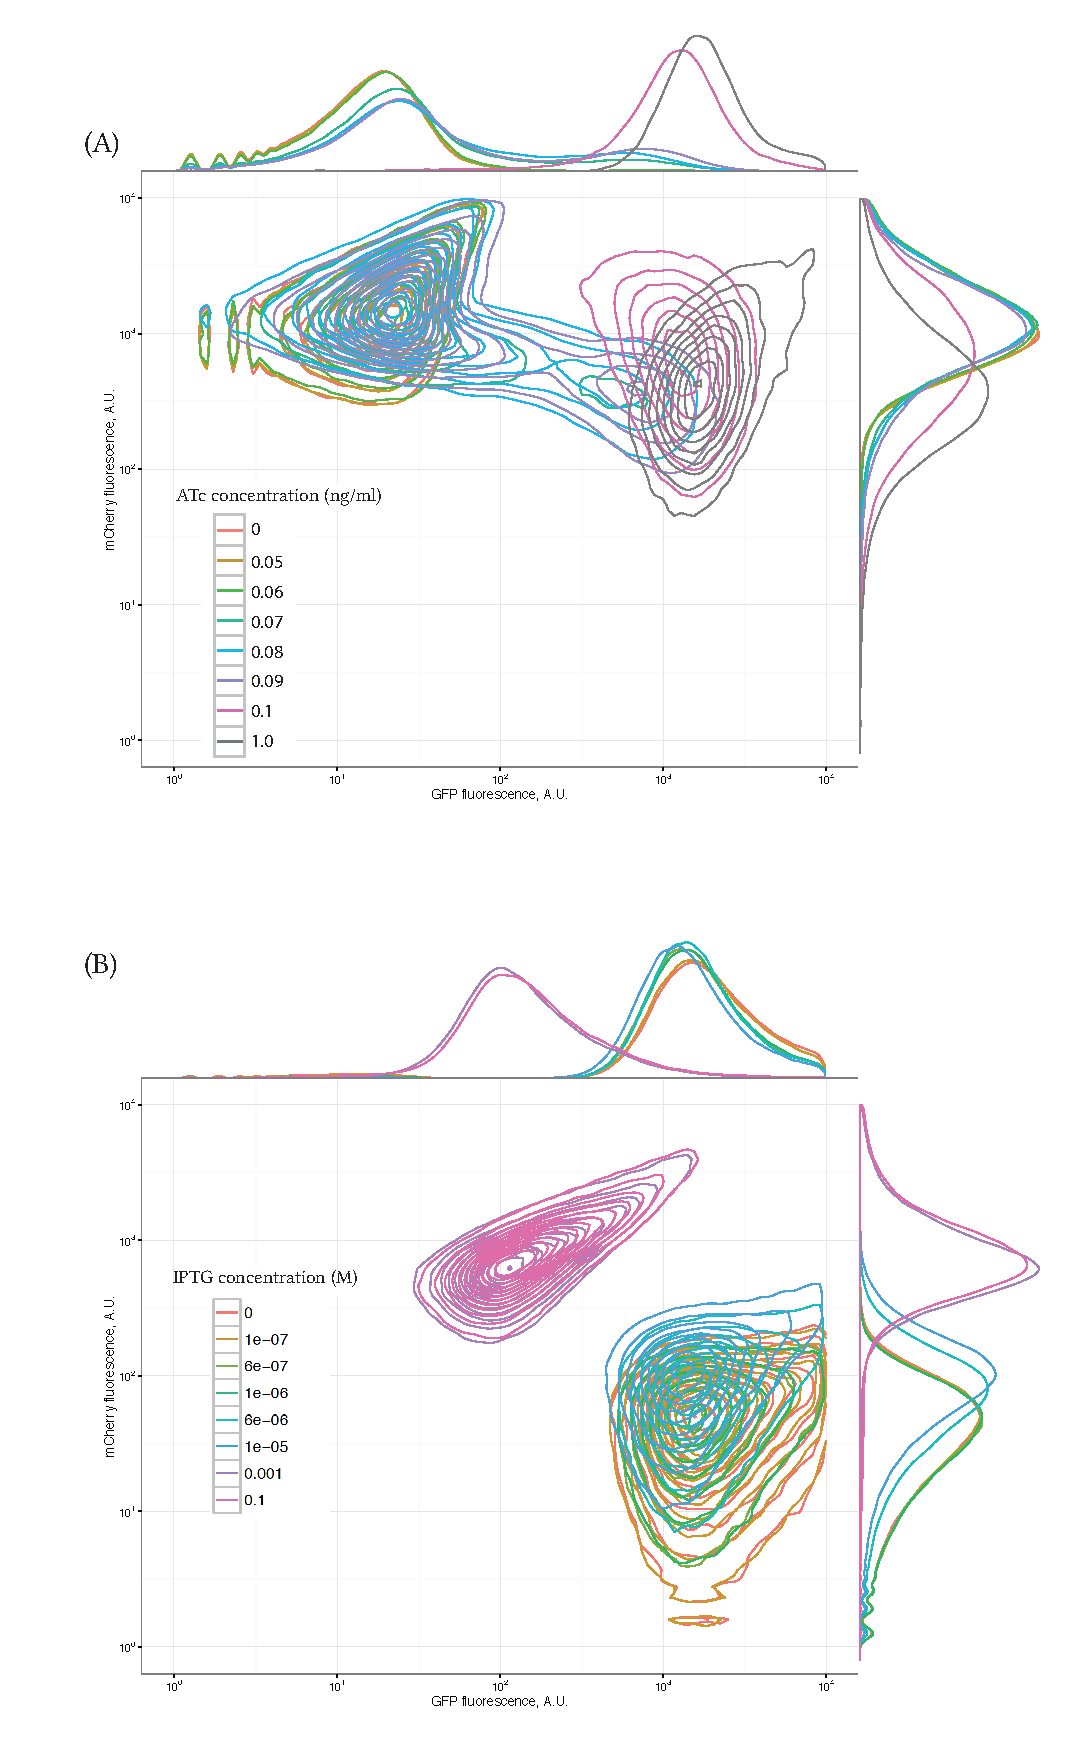
\includegraphics[scale=0.7]{chapterCharacterisation/images/pKDL071_concentrations_2d1d.png}
\caption[LoF caption]{\label{fig:switch_concent2d1d}: (A) \acrshort{atc} induction at various concentrations (B) \acrshort{iptg} induction at various concentrations. }
\end{center}
\end{figure*}
\clearpage

By taking into account the two induction curves of the switch turning to each high state, we can see the dynamic ranges of pKDL071 in \textit{E.coli}. We can see in Figure~\ref{fig:switch_concentrations_model} there is an approximately 100-fold change in fluorescent units during \acrshort{iptg} and \acrshort{atc} induction. 

 A Hill function was used to model the characterisation curves shown in Figure~\ref{fig:switch_concentrations_model}. The model used is the following:
 \begin{align}
 	F = Pmin + (Pmax - Pmin)\frac{\Big(\frac{[I]}{Kd}\Big)^n}{1+\Big(\frac{[I]}{Kd}\Big)^n},
 \end{align}
 
where F is the median fluorescent unit and [I] is the concentration of inducer. Pmin and Pmax are the minimum and maximum fluorescence respectively, and Kd and n are the dissociation constant, and Hill coefficient. I fit Hill function models using maximum likelihood estimation to the response curves. The values for parameters Pmin, Pmax, Kd, and n are 8, 1600, 0.1, 1.8 respectively for the \acrshort{atc} induction and 8, 700, 0.08, 2.5 for \acrshort{iptg} induction. 

\begin{figure*}[tb]
	\begin{center}
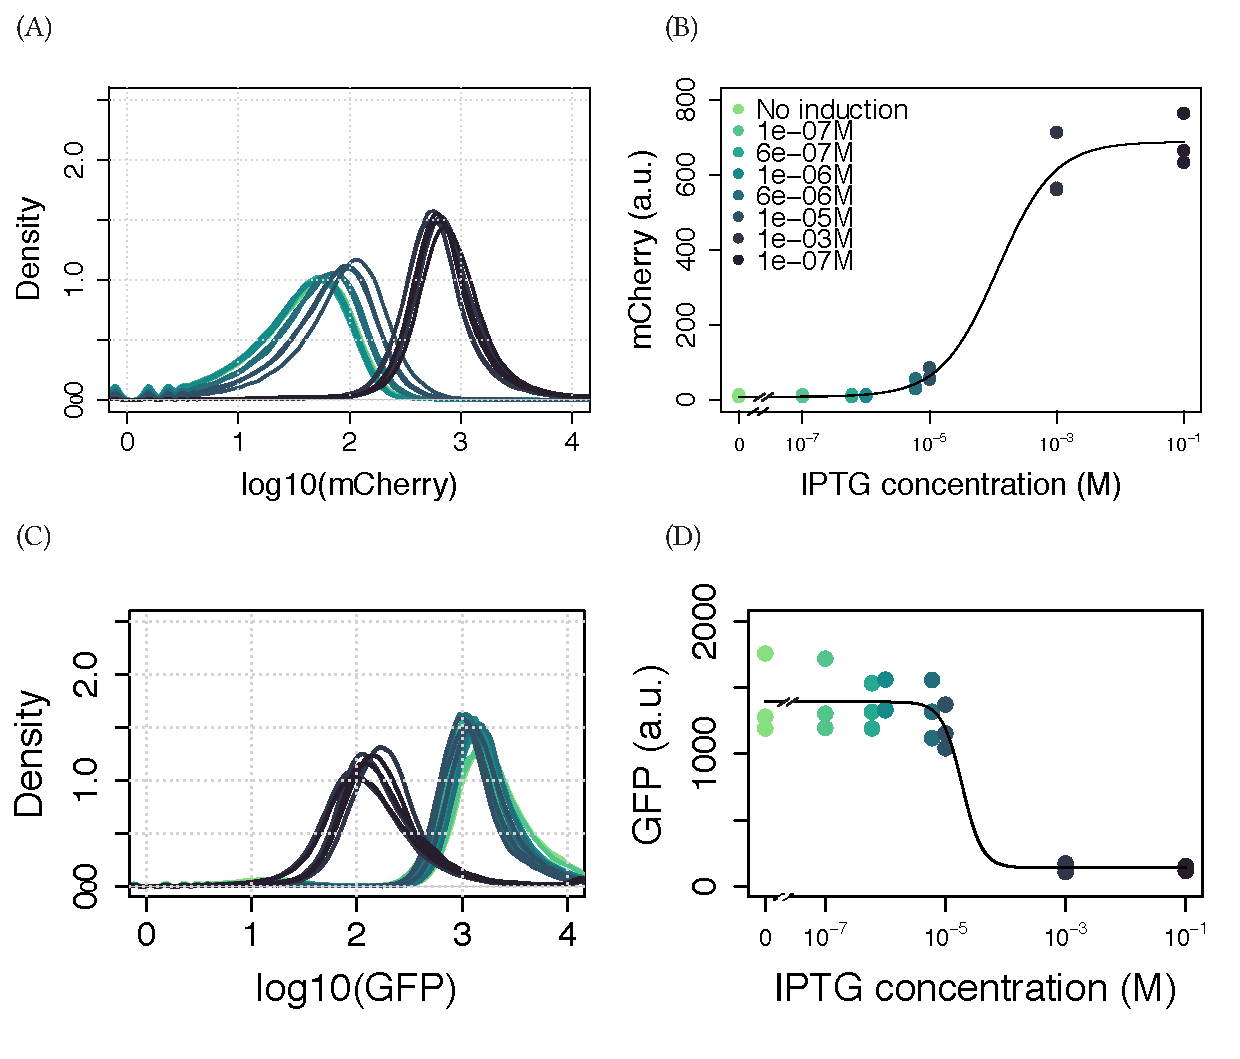
\includegraphics[width=\textwidth]{chapterCharacterisation/images/pKDL071_concentrations_model_fit.png}
\caption[LoF caption]{\label{fig:switch_concentrations_model}: (A, B) \acrshort{atc} induction of pKDL071. (C, D) \acrshort{iptg} induction of pKDL071.}
\end{center}
\end{figure*}


For the case of the \acrshort{atc} induction we observe a sharp switch between the GFP low to the GFP high state, as can be seen in the characterisation curve in Figure~\ref{fig:switch_concentrations_model}B. This is a clear indication of the bistability of this switch.

\clearpage





\subsection{Toggle switch time course assay}
\label{sec:ts_time}
I further analysed the pKDL071 toggle switch by investigating the time it takes for it to switch from one high state to the other. To do that I used the method outlined in Section~\ref{sec:flo_time}. I obtained separate time courses for the \acrshort{iptg} and \acrshort{atc} inductions. 

As can be seen in Figure~\ref{fig:switch_timecourse_atc} pKDL071 \acrshort{atc}  induction begins switching 1 hour after induction. Complete induction is seen at 6 hours. During the \acrshort{iptg} induction (Figure~\ref{fig:switch_timecourse_iptg}) we see a bimodal distribution at 4 hours, and induction is complete at 6 hours. We observe that during \acrshort{atc} induction there is an increase in \acrshort{gfp} fluorescence and a decrease in mCherry fluorescence, in the case of \acrshort{iptg} induction the increase in mCherry fluorescence is not as prominent. A decrease in GFP fluorescence is observed during \acrshort{iptg} induction. 

\begin{figure*}[tb]
	\begin{center}
\includegraphics[scale=0.7]{chapterCharacterisation/images/pKDL071_atc_time.png}
\caption[LoF caption]{\label{fig:switch_timecourse_atc}: \acrshort{atc} induction of pKDL071 over time}
\end{center}
\end{figure*}


\begin{figure*}[tb]
	\begin{center}
\includegraphics[scale=0.7]{chapterCharacterisation/images/pKDL071_iptg_time.png}
\caption[LoF caption]{\label{fig:switch_timecourse_iptg}: \acrshort{iptg} induction of pKDL071 over time}
\end{center}
\end{figure*}
\clearpage


%\begin{figure*}[tb]
%	\begin{center}
%\includegraphics[scale=0.5]{chapterCharacterisation/images/atc_timecourse.png}
%\caption[LoF caption]{\label{fig:atc_timecourse}: \acrshort{atc} induction of pKDL071 over time}
%\end{center}
%\end{figure*}
%
%\begin{figure*}[tb]
%	\begin{center}
%\includegraphics[scale=0.5]{chapterCharacterisation/images/iptg_timcourse.png}
%\caption[LoF caption]{\label{fig:iptg_timecourse}: \acrshort{iptg} induction of pKDL071 over time}
%\end{center}
%\end{figure*}
%\clearpage





%% Chapter-4 StabilityFinder ----------------------------------%%
\mainmatter*
\chapter{Modelling switches}

\section{Parameter scan}
\subsection{Background}
\subsection{Methods}
\subsection{Results}

\section{Bayesian approach to model stability}
\subsection{Background}
Synthetic biology is now entering an age where simple synthetic circuits have been built, such as toggle switches \autocite{Gardner:2000vha, Kramer:2004kq, Isaacs:2003ht, Ham:2008hh, Deans:2007cya, Friedland:2009ce}, oscillators~\autocite{Stricker:2008jqa, Fung:2005jd, Tigges:2009jx} and pulse generators~\autocite{Basu:2004gn}, but larger circuits have proven more difficult \autocite{XXX}. The leap from building low-level circuits to assembling them into complex networks has yet to be made successfully~\autocite{Lu:2009ez}, and predictable circuit behaviour remains challenging \autocite{XXX}. Efforts to do so are plagued by intra-circuit crosstalk and incompatibility, as well as cellular noise, which can render synthetic networks non-functional \textit{in vivo} \autocite{XXX}. 
\par
A circuit must be robust to a fluctuating cellular environment and its response and sensitivity must be able to be fine tuned in order to orchestrate a network of circuits that function together. A robust circuit can tolerate the compound stochasticity that a chain of circuits brings, and fine tuning of its response and sensitivity enables the researcher to make it sensitive to an upstream signal as well as influence a downstream subsystem. Parts can be fine tuned by developing component libraries~\autocite{Lu:2009ez,}, but this will be of little use if the required parameter ranges for parts to make a functional complex network are unknown, and will only perpetuate the cycles of trial-and-error. A computational method to find the range of parameter values that will produce the behaviour of choice is crucial to the design process by enabling the informed selection of appropriate parts from the libraries. If it is known that gene expression must be low for a given stability, one can select a weak promoter or a low copy plasmid for the desired construct. 
\par
Both analytical and computational approaches have been deployed for the study of the toggle switch. Analytical approaches are limited to simpler models and thus require a number of assumptions to be made. The system under consideration has to be reduced to very few equations and parameters in order to make the system solvable. This requires assumptions to be made about the system that cannot always be justified, such as the quasi-steady state approximation (QSSA). The QSSA assumes that the binding/unbinding processes are much faster than any other process~\autocite{Loinger:2007vma}, thus the bound intermediate is assumed to always be in steady state. The QSSA assumption is met \textit{in vitro} but often does not hold \textit{in vivo} and its misuse can lead to large errors and incorrectly estimated parameters~\autocite{Pedersen:2007ke}. Moreover, it is generally not possible to solve even simple stochastic models analytically, and these methods are restricted to deterministic models. The computational and graph-theoretic approaches developed for the study of multistationarity generally focus on deciding on whether a given system is incapable of producing multiple steady states ~\autocite{Conradi:2007jo, Banaji:2010fh,Feliu:2013dz}. For example, ~\textcite{Feliu:2013dz} developed an approach using chemical reaction theory and generalised mass action modelling \autocite{Feliu:2013dz}. No approach exists that can handle both deterministic and stochastic systems in an integrated manner.
\par
Here we present a computational framework based on sequential Monte Carlo that takes a model and determines whether it is capable of producing a given number of (stable) steady states and the parameter space that gives rise to the behaviour. Uniquely, this can be done for both deterministic and stochastic models, and also complex models with many parameters, thus removing the need for simplifying assumptions. Our framework can be used for comparing the conclusions drawn by various modelling approaches and thus provides a way to investigate appropriate abstractions. We have made this framework into a python package, called StabilityFinder. This methodology is used to investigate genetic toggle switches and uncover the design principles behind making a bistable switch, as well as those necessary to make a tristable switch. We find that degradation rates of transcription factors are important for bistability, and that the addition of positive autoregulation can create tristable behaviour and also significantly more robust bistability when feedback strength is well balanced. Modelling transcription and translation allows us to conclude that transcriptional bursting can inhibit bistability, and also that bistability can occur even when the assumptions of time scale separation in the repressor dynamics are not met. We also examine the design principles behind the design of bistable versus tristable switches and highlight the importance of including stochastic dynamics when modelling these systems. Finally we demonstrate the ability of the framework to examine more complex systems and examine the design principles of a three gene switch. These examples demonstrate that StabilityFinder will be a valuable tool in the future design and construction of novel gene networks. 

\subsection{Methods}
%\subsubsection{StabilityFinder}

The framework is based on a statistical inference method which combines \acrfull{abc} with \acrfull{smc} \autocite{Toni:2009tr}. This simulation-based method uses an iterative process to arrive at a distribution of parameter values that can give rise to observed data or a desired system behaviour \autocite{Barnes:2011hh}.
\acrshort{abc} methods are used for inferring the posterior distribution in cases where it is too computationally expensive to evaluate the likelihood function. Instead of calculating the likelihood, \acrshort{abc} methods simulate the data and then compare the simulated and observed data through a distance function \autocite{Toni:2009tr}. Given the prior distribution $\pi(\theta)$ we can approximate the posterior distribution, $\pi(\theta\mid x)\propto f(x\mid\theta)\pi(\theta)$, where $f(x\mid\theta)$ is the likelihood of a parameter, $\theta$, given the data, $x$. There are a number of different variations of the \acrshort{abc} algorithm depending on how the the approximate posterior distribution is sampled. 
\par
The simplest \acrshort{abc} algorithm is the \acrshort{abc} rejection sampler~\autocite{Pritchard:1999td}. In this method, parameters are sampled from the prior and data simulated thorough the data generating model. For each simulated data set, a distance from that of the desired behaviour is calculated, and if greater than a threshold, $\epsilon$, the sample is rejected, otherwise it is accepted. 
\begin{algorithm}[H]
	\label{alg:ABC}
  \caption{ABC rejection algorithm}
 \begin{algorithmic}[1]
    \Statex
	\State Sample a parameter vector $\theta$ from prior $\pi(\theta)$
	\State Simulate the model given $\theta$
    \State Compare the simulated data with the desired data, using a distance function $d$ and tolerance $\epsilon$. if $d \leq \epsilon$, accept $\theta$ 
   
  \end{algorithmic}
\end{algorithm}
\noindent The main disadvantage of this method is that if the prior distribution is very different from the posterior, the acceptance rate is very low~\autocite{Toni:2009tr}. An alternative method is the \acrshort{abc} \acrfull{mcmc} developed by~\textcite{Marjoram:2003up}~\autocite{Marjoram:2003up}. The disadvantage of this method is that if it gets stuck in an area of low probability it can be very slow to converge~\autocite{Sisson:wf}. 
The method used here is based on sequential Monte Carlo, which avoids both issues faced by the rejection and MCMC methods. It propagates the prior through a series of intermediate distributions in order to arrive at an approximation of the posterior. The tolerance, $\epsilon$ for the distance of the simulated data to the desired data is made smaller at each iteration. When $\epsilon$ is sufficiently small, the result will approximate the posterior distribution~\autocite{Toni:2009tr}.  
\par
To investigate the multistable behaviour of systems, a number of extensions to existing approaches are required. For a given set of parameter values, sample points are taken across initial conditions using latin hypercube sampling \autocite{XXX}, and the ensemble system simulated in time until steady state. The distance function in \acrshort{abc} is replaced by a distance on the desired stability of the simulated model. To do this we cluster the steady state coordinates using k means clustering and use the gap statistic to determine the number of clusters \autocite{XXX}. The algorithm is summarised below.
\begin{algorithm}[H]
\label{alg:StabilityFinder}
\caption{StabilityFinder algorithm}
 \begin{algorithmic}[1]
    \Statex
	\State Initialise $\epsilon$ 
	\Let{population p}{1}
	\If{p $= 1$}
		\State Sample particles ($\theta$ ) from priors
		\Else
			\State Sample particles from previous population
			\State Perturb each particle by $\pm$ half the range of the previous population (j) to obtain new perturbed population (i).
	\EndIf
	\State Sample initial conditions via Latin Hypercube Sampling.
    \State Simulate each particle to obtain steady state values.
    \State Cluster steady state
	\State Reject particles if d $\textgreater$ $\epsilon$.
    \State Calculate weight for each accepted $\theta$
	%\State $w_{t}^{(i)} = \begin{cases} 1, & \mbox{if } p = 0 \\\frac{\pi(\theta_{t}^{(i)})}{\sum_{j=1}^N w_{t-1}^{(j)} K_{t}(\theta_{t-1}^{(j)}, \theta_{t}^{(i)})}, and \mbox{if } p \geq  0. \end{cases}$
	\State Normalise weights
	\Repeat{steps 3 - 15} \Until{$\epsilon \leq \epsilon_T$}
  \end{algorithmic} 
\end{algorithm}
\noindent This algorithm is available as a Python package, called StabilityFinder. %which is available at \url{https://github.com/ucl-cssb/StabilityFinder.git}.  
The user provides an SBML model file \autocite{XXX} and an input file that contains all the necessary information to run the algorithm, including the desired stability and the final tolerance, $\epsilon$, for the distance from the desired behaviour necessary for the algorithm to terminate. The flow of execution is illustrated in Figure~\ref{fig:fig1}. Since the algorithm is computationally intensive, all deterministic and stochastic simulations are performed using algorithms implemented on \acrfull{gpu}s \autocite{XXX}.

\subsection{Testing StabilityFinder}

\textcite{Gardner:2000vha} constructed the first synthetic genetic toggle switch~\autocite{Gardner:2000vha}. Their model consisted of two mutually repressing transcription factors, as shown in Figure~\ref{fig:fig2}A, and in the deterministic case is defined by the following \acrshort{ode}s.
\begin{align*}
\frac{du}{dt} &= \frac{a_1}{1+v^{\beta}} - u\\
\frac{dv}{dt} &= \frac{a_2}{1+u^{\gamma }} - v,
\end{align*}
where \textit{u} is the concentration of repressor 1, \textit{v} the concentration of repressor 2, $a_1$ and $a_2$ denote the effective rates of synthesis of repressors 1 and 2 respectively,  \textit{$\beta$} is the cooperativity of repression of promoter 1 and \textit{$\gamma$} of repressor 2. Gardner \textit{et al} studied the deterministic case and concluded that there are two conditions for bistability for this model; that $a_1$ and $a_2$ are balanced and that $\beta$, $\gamma$ \textgreater 1 \autocite{Gardner:2000vha}. In order to test StabilityFinder we used it to find the posterior distribution for which this model exhibits bistable behaviour. We therefore set the desired behaviour to two (stable) steady states, and using a wide range of values as priors as shown in the Supplementary Information, we used StabilityFinder to find the parameter values necessary for bistability to occur. The posterior distribution calculated by StabilityFinder for the Gardner deterministic case is shown in Figure~\ref{fig:fig2}B.
\par
These results agree with the results reported by~\textcite{Gardner:2000vha}~\autocite{Gardner:2000vha}. For this switch to be bistable $a_1$ and $a_2$ must be balanced while $\beta$ and $\gamma$ must both be \textgreater 1, as can be seen in the marginal distributions of $\beta$ and $\gamma$ in Figure~\ref{fig:fig2}B. The conditions set by the original paper for parameters $a_1$ and $a_2$ are met, as the joint distribution shown in Figure~\ref{fig:fig2}B matches the bifurcation lines calculated in the original paper {\color{red} How do you know, did you calculate these? I think you should try and plot them on the posterior}. 
We next applied StabilityFinder to the case of the Gardner switch under stochastic dynamics using the same priors as the deterministic case, and again searched the parameter space for bistable behaviour. The posterior is shown in Figure~\ref{fig:fig2}C. We can see that the conditions on the parameters required for bistability in the deterministic case generally still stand in the stochastic case. There appears to be slightly looser requirements on the parameters of the stochastic model (wider marginal distributions), which is expected due to the nature of clustering deterministic steady states versus stochastic steady states. The gap statistic is used in the case of the stochastic case, as it is capable of dealing with noisier data whereas a simpler and faster algorithm is used for clustering the deterministic solutions. The study on the effect of the clustering methods on robustness is shown in the Supplementary Information. These results demonstrate that StabilityFinder can be used to find the parameter values that can produce a desired stability and allow us to confidently apply the methodology to more complex models.

\begin{table}[h]
\centering
\caption{Gardner switch priors in the deterministic and stochastic cases}
\label{tab:gard_det_stoch}
\begin{tabular}{@{}cccccc@{}}
\toprule
\multicolumn{4}{c}{Parameters}                          & \multicolumn{2}{c}{Species} \\ \cmidrule(lr){1-4}
\cmidrule(lr){5-6}
$a_1$ & $\beta$ & $a_2$ & \multicolumn{1}{c}{$\gamma$} & $s_1$        & $s_2$        \\
0-60  & 0-5     & 0-60  & 0-5                           & 0-100        & 0-100        \\ \bottomrule
\end{tabular}
\end{table}


\subsection{Calculating robustness}

We calculate robustness $R$ by using a Monte Carlo sampling rejection algorithm by taking random samples from the prior and accepting those found in the functional region $F$. Robustness is then defined as the number of accepted samples divided by the total number of samples.

 In order to test this algorithm we use a cube of equal length sides as the prior. Instead of a posterior distribution we draw random samples from uniform $u(a, b)$ in three dimensions or multivariate normal $N(\mu, \sigma)$ distribution. In the case of the uniform distribution, we adjust the range of the data by drawing samples from a range incrementally smaller than the prior cube, always centred in the centre of the prior cube. In the case of a normal distribution $\mu$ is set to the centre of the cube and we vary $\sigma$ to get a distribution with increasingly larger range, approaching the full range of the prior.  

 We calculate the true robustness $R_t$ by calculating the ratio of the volume of the data to the volume of the prior cube. In the case where data$~u(a, b)$, the data is treated as a cube with length $a = (b - a)$ and volume $V = a^3$. In the case where data$~N(\mu, \sigma)$, the data is treated as a sphere with radius $r = \frac{(max - min)}{2}$ and volume $V = \frac{4}{3} * \pi * r^2$. 
 
\begin{algorithm}[H]
	\label{alg:robustness}
  \caption{Calculating robustness via Monte Carlo sampling rejection}
 \begin{algorithmic}[1]
    \Statex
    \Let{$R$}{Robustness}
    \Let{$F$}{Functional region}
    \For{Each variance sample}
    	\State Generate data set
    	\State Calculate true $R_t$: 
    	\Let{$V_p$}{Prior Volume}
    	\Let{$a_p$}{Prior max - min} \
    	\State $V_p = a_p^3$ 
    	
    	\If{data$~N(\mu, \sigma)$}
    		\State Get min and max of data \
    		\Let{r}{$\frac{max - min}{2}$} \
    		\State $V_d = \frac{4}{3} * \pi * r^2$ 
    	\EndIf
    	
    	\If{data$~u(min, max)$}
    		\Let{$a$}{$max - min$} \
    		\State $V_d = a^3$
    		\State $R_t = \frac{V_d}{V_p}$
    	\EndIf
    	
    	\State Define grid
    	\State Do \acrfull{kde} on data
    	\For{Each repeat}
    		\State Sample from priors 
    		\Let{$Z$}{5th percentile of KDE}
    		\Let{$F$}{KDE > $Z$}
    		\If{sample $\in$ grid}
    		\State Find sample's position in grid
				\If{position $\in$ $F$}
    				\State $accepted += 1$
    			\EndIf
    		\EndIf
    		\State $R$ = $\frac{accep
    	ted}{number of samples}$
    	\EndFor

  \EndFor  
   \State \Return mean($R$), standard deviation($R$), $R_t$
  \end{algorithmic}
\end{algorithm}	

\clearpage


\subsubsection{Normal distribution}


\begin{figure}[htbp]
\centering
\includegraphics[scale=0.6]{chapterStabilityFinder/images/robustness_calc_norm.png}
\caption[LoF caption]{}
\label{}
\end{figure}
\clearpage
\paragraph{Studying the effect of correlation}
\begin{figure}[htbp]
\centering
\includegraphics[scale=0.6]{chapterStabilityFinder/images/normal_correl.png}
\caption[LoF caption]{}
\label{}
\end{figure}
\clearpage
\paragraph{Comparing increasing dimensions}
\begin{figure}[htbp]
\centering
\includegraphics[scale=0.6]{chapterStabilityFinder/images/robustness_s_normal_dimens.pdf}
\caption[LoF caption]{}
\label{}
\end{figure}
\clearpage
\subsubsection{Uniform distribution}
\begin{figure}[htbp]
\centering
\includegraphics[scale=0.6]{chapterStabilityFinder/images/robustness_calc_unif.png}
\caption[LoF caption]{}
\label{}
\end{figure}
\clearpage
\paragraph{Comparing increasing dimensions}
\begin{figure}[htbp]
\centering
\includegraphics[scale=0.6]{chapterStabilityFinder/images/robustness_s_uniform_dimens.pdf}
\caption[LoF caption]{}
\label{}
\end{figure}
\clearpage


\subsection{Lu toggle switch models}

We next analyzed an extension of the Gardner switch model developed by~\textcite{Lu:2014kc}~\autocite{Lu:2014kc}. They considered two types of switches, the classic switch consisting of two mutually repressing transcription factors (model \acrshort{cs-lu}), as well as a \acrfull{dp-lu}.  The classical switch was found to be bistable given the set of parameters used, while the DP switch was found to be tristable ~\autocite{Lu:2014kc}. The classical model used in their study is given by the following system of \acrshort{ode}s.
\begin{align*}
\dot{x} & = g_{x}\, H^{S}_{xy}(y) -k_{x}x \\
\dot{y} & = g_{y}\,H^{S}_{yx}(x) -k_{y}y,
\end{align*}
where
\begin{align*}
H^{S}_{I}(x) &= H^{-}_{I}(x)+\lambda_{I}H^{+}_{I}(x) \\
H^{-}_{I}(x) &= 1 \big/\left[1+(x/x_{I})^{n_{I}}\right] \\
H^{+}_{I}(x) &= 1-H^{-}_{I}(x),
\end{align*}
and $g_I$ represents the production rate, $k_I$ the degradation rate, $n_I$ the Hill coefficient, $x_I$ the Hill threshold concentration and $\lambda_I$ the fold change of the transcription rates, and $I\in\{xy, yx, xx, yy\}$. 
\par
For the parameter values used in the Lu study, the classical switch exhibits three steady states (Figure~\ref{fig:fig3}), two of which are stable and one is unstable. Using StabilityFinder with priors centred around the parameter values used in the original paper (see Supplementary Information), we can identify the most important parameters for achieving bistability. The posterior distribution of these models are shown in Figure~\ref{fig:fig3}A. We find that the parameters representing the rates of degradation of the transcription factors in the system ($k_x$,$k_y$) must both be large in relation to the prior ranges for bistability to occur. Protein degradation rates have been shown to be important for many system behaviours including oscillations \autocite{XXX}. {\color{red} Anything else regarding this classical model? with more parameters}

It is known that that the addition of positive autoregulation to the classical toggle switch can induce tristability  \autocite{XXX, Lu:2014kc}. Here we investigate the interplay of positive autoregulation on the values of the other parameters in the model. We extended the analysis presented in ~\textcite{Lu:2014kc} by including the switch with single positive autoregulation (model \acrshort{sp-lu}), where an asymmetry of positive feedbacks is present between the two genes. The advantage of using StabilityFinder over solving the system analytically is that the full parameter space is explored rather than solving the system for a single set of parameters. This allows us to deduce model properties that could not otherwise be identified. Robustness to parameter fluctuations can be explored, as well as parameter correlations and restrictions on the values they can take while still producing the desired behaviour.  
\par
The \acrshort{dp-lu} model is given by
\begin{align*}
\dot{x} = f_{x}(x,y) &= g_{x}\, H^{S}_{xy}(y)\, H^{S}_{xx}\,(x)-k_{x}x \\
\dot{y} = f_{y}(x,y) &= g_{y}\,H^{S}_{yx}(x)\,H^{S}_{yy}\,(y)-k_{y}y,
\end{align*}
whereas the \acrshort{cs-lu} switch is modelled using the following \acrshort{ode} system
\begin{align*}
\dot{x} & = g_{x}\, H^{S}_{xy}(y)\, H^{S}_{xx}\,(x)-k_{x}x \\
\dot{y} & = g_{y}\,H^{S}_{yx}(x) - k_{y}y.
\end{align*}
We find that the switch with single positive autoregulation is capable of bistable behaviour as seen in Figure~\ref{fig:fig3}B, but this is only possible when the strength of the promoter under positive autoregulation, $gx$, is small. There appear to be no such constraints on the strength of the original, unmodified, promoter, $gy$.  
\par
Upon examination of the \acrshort{dp-lu} model, we also find that tristability in the switch is relatively robust, as tristability is found across a large range of parameter values, with no parameters strongly constrained {\color{red} Can we say a bit more here?}. Two types of tristable behaviour are identified, one where the third steady state is at (0,0) and and one where the third steady state has non-zero values. This result agrees with previous work by~\textcite{Guantes:2008gs}, who found that a switch can exhibit two kinds of tristability, one in which the third steady state is high (\RNum{3}$_H$) and one in which it is low (\RNum{3}$_L$)~\autocite{Guantes:2008gs}. %The difference between the two tristable switches is explored in a later section. 

deterministic dynamics~\autocite{Guantes:2008gs}. The classical switch is also capable of both bistable and tristable behaviour when stochastic dynamics capture small number effects~\autocite{Ma:2012dt}. It is therefore of great interest to understand the conditions under which these two behaviours occur in both stochastic and deterministic scenarios. 
\par
In order to do this using StabilityFinder, we first obtained posterior distributions for bistable and tristable behaviours in the deterministic case (\acrshort{dp-lu} model) and then compared the individual parameter distributions (Figure~\ref{fig:fig6} and Supplementary Information). From analysis of the one dimensional marginal distributions it appears that there is no difference in the parameter values that allow a switch to be bistable versus tristable (Figure~\ref{fig:fig6}B). However, upon examination of the two dimensional marginal distributions we find that the correlation structure of a small subset of the posterior parameter values is in fact different under the two behaviours (Figure~\ref{fig:fig6}C). Most notably, we find differences in the bivariate distribution of the two parameters for gene expression, $gx$ and $gy$, as highlighted in Figure~\ref{fig:fig6}C, box 1. In the tristable case the distribution is more constrained than in the bistable case, as both parameters must be small for tristability to arise. 
Parameters $xYY$ and $gy$ are tightly constrained in the tristable case and both required to be small, but less so in the bistable case (Figure~\ref{fig:fig6}C, box 3). Another notable difference is between parameters $xXX$ and $lXX$ shown in Figure~\ref{fig:fig6}C, box 4, where they are constrained in the bistable case but not the tristable case. Interestingly, we also find parameter correlations conserved between the bistable and tristable case, as seen in Figure~\ref{fig:fig6}C, box 2, where parameters $lXX$ and $gx$, positive autoregulation and gene expression are negatively correlated in both cases.  This highlights the importance of treating unknown parameters as distributions rather than fixed values when studying the parameter values of a model, as they are capable of uncovering not only the ranges and values needed but also the correlations between parameters that would not have otherwise been detected.

To further demonstrate the flexibility of our framework we investigated a system capable of higher stabilities. Multistability is found in differentiating pathways, like the myeloid differentiation pathway~\autocite{Ghaffarizadeh:2014bt, Cinquin:2005go}. We allow for these more complex dynamics by extending the Lu DP model by adding another gene, making it a three gene switch.  This new system is depicted in Figure~\ref{fig:fig8}A. In StabilityFinder we look for six steady states, the output being in nodes $X$ and $Y$ and using the priors shown in Table~\ref{tab:multi_priors}. We successfully find that the system is capable of six steady states, as shown in Figure~\ref{fig:fig8}C and as predicted mathematically and shown in Figure~\ref{fig:fig8}B. Interestingly, and consistent with the results presented above, we find that the most constrained parameters for this behaviour are again the degradation rate of the proteins, $kx$. Additionally we find that the Hill coefficients for the repressors, $nxy$, are tightly contrained to be smaller than 1.5 as seen in Figure~\ref{fig:fig8}D. {\color{red} What else can we do here? Can we simulate the system switching or something?} This example demonstrates that StabilityFinder can be used to elucidate the dynamics of more complex network architectures, which will be key to the successful design and construction of novel gene networks as synthetic biology advances.

\begin{table}[htpb]
\centering
\caption{Priors of the classical(\acrshort{cs-lu}), single positive (\acrshort{sp-lu}) and double positive (\acrshort{dp-lu}) models.}
\label{tab:lu_all}
\begin{tabular}{@{}ccccc@{}}
\toprule
Parameter                                            & Symbol & \acrshort{cs-lu}       & \acrshort{sp-lu}        & \acrshort{dp-lu}       \\ \midrule
\multirow{2}{*}{Production rate}                & gx        & 30-50   & 1-2       & 1-100    \\
                                                & gy        & 30-50   & 20-25     & 1-100    \\[4pt]
\multirow{2}{*}{Degradation rate}               & kx        & 0-0.5   & 50-55     & 0-1      \\
                                                & ky        & 0-0.5   & 48-52     & 0-1      \\[4pt]
\multirow{2}{*}{Hill coefficient}               & nxy       & 1-5     & 30-35     & 0-10     \\
                                                & nyx       & 1-5     & 0.1-0.2   & 0-10     \\[4pt]
\multirow{2}{*}{Hill thresholds concentration}  & xxy       & 100-300 & 2-3       & 100-1000 \\
                                                & xyx       & 100-300 & 0.4-0.6   & 100-1000 \\[4pt]
\multirow{2}{*}{Transcription rate fold change} & lxy       & 0-0.5   & 0.02-0.04 & 0-1      \\
                                                & lyx       & 0-0.5   & 0.02-0.04 & 0-0.2    \\[4pt]
\multirow{2}{*}{Hill coefficient}               & nXX       & -       & 25-30     & 0-10     \\
                                                & nYY       & -       & 0.01-0.02 & 0-10     \\[4pt]
\multirow{2}{*}{Hill thresholds concentration}  & xXX       & -       & 0.4-0.5   & 50-500   \\
                                                & xYY       & -       & 1-3       & 50-500   \\[4pt]
\multirow{2}{*}{Transcription rate fold change} & lXX       & -       & 65-72     & 1-20     \\
                                                & lYY       & -       & 0.02-0.04 & 1-20     \\ \hline
\end{tabular}
\end{table}


\begin{table}[htpb]
\centering
\caption{Priors used in the three-node switch}
\label{tab:multi_priors}
\begin{tabular}{@{}ccc@{}}
\toprule
Parameter                           & Symbol & Range   \\ \midrule
Production rate                & gx        & 3-5    \\
Degradation rate               & kx        & 0-0.2     \\
Hill coefficient               & nxy       & 0-2    \\
Hill thresholds concentration  & xxy       & 140-160 \\
Transcription rate fold change & lxy       & 0-0.2     \\
Hill coefficient               & nxx       & 2-4     \\
Hill thresholds concentration  & xxx       & 90-110  \\
Transcription rate fold change & lxx       & 8-12    \\ \bottomrule
\end{tabular}
\end{table}


\subsection{Mass Action switches}						
Although the DP switch can achieve tristability, we investigated how the addition of positive autoregulation alters the robustness of the switch for bistable behaviour. Here we define a robust system as a device that can withstand fluctuations in parameter values and still produce the desired behaviour (parametric robustness). Feedback loops are well known key regulatory motifs~\autocite{Brandman:2005ci}. Although negative feedback loops are essential for homeostasis and buffering~\autocite{Thomas:1995id} and can increase robustness to extrinsic noise sources, we focussed on the addition of positive feedback because this has been shown to increase robustness in other systems \autocite{XXX}. We use StabilityFinder to compare the two models, and determine whether its worthwhile building a bistable circuit with added positive feedback.
%StabilityFinder allows us to study more complex systems and to take stochasticity into account. This is relevant in a biological systems in which realistic models tend to involve many species and interactions and where small molecule numbers and external noise are non negligible. 
\par
In order to study the switch system in the most realistic way, we avoid using the quasi-steady state approximation (QSSA) that is often used in modelling the toggle switch. Using mass action, this changes the two-equation system used in~\textcite{Lu:2014kc}~\autocite{Lu:2014kc} into a system of 18 equations and 7 parameters in the classical switch case. These are shown in the Supplementary Information.% Using mass action, the two models representing the  C switch with no autoregulation and DP switch are shown in Figure~\ref{fig:fig4} {\color{red} No they're not}.  

Given the posterior distributions shown in Figure~\ref{fig:fig4}, we find that the parameter for transcription factor degradation ($deg$) has to be high, a result that reflects the findings for the Lu models above {\color{red} Do we really see that??}. We also find that the addition of positive feedback loops greatly increases the system's robustness to parameter fluctuations as seen in Figure~\ref{fig:fig4}D. Adding positive feedback loops to the model allows it to be bistable over a greater range of parameter values, but only when the system is symmetric. When this constraint is removed we no longer see a difference in robustness between the CS-MA and DP-MA models. {\color{red} What does this mean? }

%This indicates that small fluctuations in parameters in the cellular environment will not affect the system's ability to be bistable, and thus makes it more suitable for use in synthetic biological applications where a very constrained parameter set can be too restrictive.% This makes it a better candidate for building new synthetic devices based on the toggle switch design.

%We identified the parameter region within which these models are bistable, information that is important when building such a device in the lab. In the future, by selecting the system components accordingly, the parameter values can be adjusted \textit{in vivo}. For example, the desired level of gene expression can be accomplished by selecting the appropriate RBS sequence~\autocite{Salis:2009gk}. Another method to modify the parameter values \textit{in vivo} is to select the promoter to have the strength corresponding to the levels of gene expression and repression desired. Activity of each promoter can be measured and standardised~\autocite{Kelly:2009bj} making this process possible. For a system requiring more than one promoter, these can be efficiently selected from a promoter library using a genetic algorithm~\autocite{Wu:2011bq}. These standardised interchangeable components with known sequence and activity~\autocite{Kelly:2009bj,Canton:2008fv} can be selected and used to construct a desired system and replicate the parameter values found using StabilityFinder.

We find that in the stochastic case, both the simple switch, S-MA, and positive autoregulation switch, DP-MA, are capable of both bistable and tristable behaviour. The fact that tristability can occur in the classical model is consistent with the effect of small molecule numbers; if gene expression remains low, it provides the opportunity for small number effects to be observed, and the third steady state to stabilise \autocite{Ma:2012dt}. In order to ensure that the tristable switches found in the stochastic case are truly tristable, we re-sample the posterior distributions and simulate to steady state. If the resulting phase plots are tristable then we know that the posterior truly represents tristability. As can be seen in Figure~\ref{fig:fig7}B, differences in the parameter values are observed between the bistable and tristable switches, in both CS-MA and DP-MA models. The design principles for both the CS-MA model and the DP-MA model are summarised in Table~\ref{tab:des_prin}

\begin{table}[]
\centering
\caption{Design principles of bistable and tristable switches}
\label{tab:des_prin}
\begin{tabular}{@{}ccccc@{}}
\toprule
                    & \multicolumn{2}{c}{\textbf{CS-MA}} & \multicolumn{2}{c}{\textbf{DP-MA}} \\ \cmidrule(l){2-3}\cmidrule(l){4-5}
                    & \textit{Bistable}    & \textit{Tristable}   & \textit{Bistable}    & \textit{Tristable}   \\\cmidrule(l){2-2}\cmidrule(l){3-3}\cmidrule(l){4-4}\cmidrule(l){5-5}
dimerisation        & High        & Low         & High        & Low         \\
protein degradation & -           & -           & -           & Low         \\
dimer degradation   & Low         & -           & Low         & -           \\\bottomrule
\end{tabular}
\end{table}

\section{Conclusions}
We have developed an algorithm that can identify the parameter regions necessary for a model to achieve a given number of stable steady states. The novelty in our framework over existing methodology is that complex models can be analyzed assuming both deterministic and stochastic dynamics. We have shown that the algorithm can be used to infer parameter ranges and compare robustness between models. We found that adding positive feedback increases the robustness of a toggle switch model to parameter fluctuations. We also found that stochastic modelling can enable a model to achieve stabilities not possible in the deterministic case. We uncovered the design principles that make a tristable switch and finally we found that a three-node switch is capable of hexastability.
\par
Tools that can identify parameter regions that give rise to specific behaviours will be key for the success of synthetic biology. In the future, by selecting the system components accordingly, the parameter values can be adjusted \textit{in vivo}. For example, the desired level of gene expression can be accomplished by selecting the appropriate RBS sequence~\autocite{Salis:2009gk}. Another method to modify the parameter values \textit{in vivo} is to select the promoter to have the strength corresponding to the levels of gene expression and repression desired. Activity of each promoter can be measured and standardised~\autocite{Kelly:2009bj} making this process possible. For a system requiring more than one promoter, these can be efficiently selected from a promoter library using a genetic algorithm~\autocite{Wu:2011bq}. These standardised interchangeable components with known sequence and activity~\autocite{Kelly:2009bj,Canton:2008fv} can be selected and used to construct a desired system and replicate the parameter values found using StabilityFinder.
\par
The methodology presented here can also be used to study the topology of more complex multistable switches that exist in natural biological systems such as developmental pathways. We also limited our framework to the objective behaviour of a given number of stable steady states. This could be extended to examine systems with a given switching rate or systems robust to a particular set of perturbations, both of which could be of great importance for building more complex genetic circuits.
\par
More generally our results highlight that changing the level of abstraction included in the model can significantly alter the observed multistationarity. This is further exacerbated by a change in the dynamics from deterministic to stochastic. These results for the case of multistationarity, assuming they translate to systemic behaviour more generally, suggest that a programme of experimental work, combined with systems modelling, is required to understand the rules of thumb for abstraction in model based design of synthetic biological systems.   

\begin{figure*}[h]
\begin{center}
\includegraphics[scale=0.9]{chapterStabilityFinder/images/figure-01.png}
\caption[LoF caption]{\label{fig:fig1}: Using sequential Monte Carlo to examine system stability. The algorithm takes as input a model (A) and evolves it to the stability of choice (C) via intermediate populations. In this example model shown in A, There are two species and two parameters. For the model to be bistable, the phase plot of the two species of interest must have two distinct densities, as shown in (C). The parameter space of the model is searched through our algorithm until the resulting simulations give rise to bistability. The parameter values for the model that demonstrated the desired behaviour are given as an output (D). The output consists of the accepted values for each parameter, as well as each density plotted against the other. This allows us to uncover correlations between parameter values. We made this algorithm into a python package, called StabilityFinder. The overview of the algorithm is shown in (E).}
\end{center}
\end{figure*}
\clearpage

\begin{figure*}[h]
\begin{center}
\includegraphics[width=\textwidth]{chapterStabilityFinder/images/figure-02.png}
\caption[LoF caption]{ \label{fig:fig2}: Elucidating the stability of the Gardner switch. The Gardner model (A) consists of two mutually repressing transcription factors. It can be reduced to a two-equation system, where $u$ and $v$ are the two transcription factors, $a_1$,$a_2$ are their effective rates of synthesis, $u$,$v$ are their concentrations and $\beta$, $\gamma$ represent the cooperativity of each promoter. There are four parameters in the model, for which we want to find the values for which this system is bistable. We use StabilityFinder to find the posterior distribution of the bistable Gardner switch, deterministically (B) and stochastically (C). The posterior distributions are shown as the density plots of each parameter as well as each one plotted against the other. }
\end{center}
\end{figure*}
\clearpage

\begin{figure*}[p]
\begin{center}
\includegraphics[width=\textwidth]{chapterStabilityFinder/images/figure-03.png}
\caption[LoF caption]{ \label{fig:fig3}: The three variants of the Lu models. (A)\textbf{CS (deterministic).}  The classic switch with no autoregulation is bistable. The most restricted parameters for this behaviour are $kx$ and $ky$ which both have to be high relative to the prior while the net protein production for $X$ and $Y$ myst be balanced. (B)\textbf{SP (deterministic).}The extended Lu model with a single positive autoregulation on $X$. This model is bistable when $gx$ is small. (C) \textbf{DP (deterministic).} The Lu model with double positive autoregulaiton is tristable, and its posterior distribution shown here. We find two types of tristable behaviour, one where the third steady state is zero-zero and one where the third state is high (non-dead).}
\end{center}
\end{figure*}
\clearpage

\begin{figure*}[h]
\begin{center}
\includegraphics[scale=0.5]{chapterStabilityFinder/images/figure-04.png}
\caption[LoF caption]{ \label{fig:fig4}: Adding positive feedback increases robustness to parameter fluctuations. We compare the posterior distributions of the simple mass action switch and the switch with added double positive autoregulation (A). The two models were both capable of bistable behaviour (B). The two posterior distributions are shown in (C). Comparing the functional region $F$ of the posterior distributions (D) we find that there is a five-fold increase in robustness when positive autoregulation is added. This is not the case for the asymmetric switch in which there is no significant difference in robustness between the CS-MA and DP-MA models.}
\end{center}
\end{figure*}
\clearpage


\begin{figure*}[h]
\begin{center}
\includegraphics[scale=0.6]{chapterStabilityFinder/images/figure-05.png}
\caption[LoF caption]{ \label{fig:fig5}: (A) Separating transcription and translation in the mass action model. (B) Transcriptional bursting does not allow for a bistable switch. (C) The Quassi Steady state approximation assumption that the dimerization reaction ($dim$) is much faster than its reverse ($dim\_r$) cannot be justified here. The median of the data (red) lies below the x=1 line (black dashed line) which indicates that in the majority of the particles in the posterior $\frac{dim}{dim\_r} < 1$  (D) No difference was found in the robustness to parameter fluctuations for the two models tested here.}
\end{center}
\end{figure*}

\begin{figure*}[h]
\begin{center}
\includegraphics[width=\textwidth]{chapterStabilityFinder/images/figure-06-alt.png}
\caption[LoF caption]{ \label{fig:fig6}: Design principles of a tristable switch. (A) Using the Lu model with added positive autoregulation we uncover the design principles dictating if a switch will be bistable or tristable. (B) By considering each parameter separately we cannot find a significant difference in the parameter values acceptable for a bistable versus a tristable switch. (C) By considering the bivariate distributions of the parameters we can uncover the differences in the parameters of a bistable switch compared to a tristable switch. The posterior distribution of the bistable switch is shown in red and of the tristable switch in blue. The bivariate distributions for which a difference is observed between a bistable and a tristable switch are in black boxes. }
\end{center}
\end{figure*}


\begin{figure*}[h]
\begin{center}
\includegraphics[scale=0.6]{chapterStabilityFinder/images/figure-07.png}
\caption[LoF caption]{ \label{fig:fig7}: Tristability is possible in the mass action toggle switch models only when simulated stochastically. (A) the simple toggle switch with no autoregulation can be both bistable and tristable. The two posteriors are shown, where the posterior distribution of the bistable switch is shown in red and of the tristable switch in blue. From the posterior distribution we can deduce the the dimerization parameter must be small for tristability to occur but large for bistability. The switch with double positive autoregulation and its posterior distributions for the bistable and tristable case are shown in (B). A sample phase plot of a stochastic tristable and bistable mass action switch is shown in (C). Comparing the robustness of the switch with and without positive autoregulation, we don't find a significant difference (D).}
\end{center}
\end{figure*}
\clearpage

\begin{figure*}[h]
\begin{center}
\includegraphics[scale=0.7]{chapterStabilityFinder/images/figure-08.png}
\caption[LoF caption]{ \label{fig:fig8}: The three-node mutual repression model, with added positive auto-regulation on each node. (A) The model. The model is studied in two dimensions using StabilityFinder, $X$ and $Y$. (B) The phase plot of the resulting final population of StabilityFinder. There are 6 steady states. (C) The posterior distribution of the 6-steady state three-node system. Parameters $kx$ and $nxy$ are the most constrained.}
\end{center}
\end{figure*}


\section{Methods}

 
 
\subsection{Calculating robustness}




\section{Results}
\subsection{Testing StabilityFinder: The Gardner toggle switch}

This toggle switch model was developed by T.~S. Gardner~\autocite{Gardner:2000vha}. This model consists of two mutually repressing transcription factors and is defined by the following ODEs:

\begin{align}
\frac{du}{dt} &= \frac{a_1}{1+v^{\beta}} - u \label{eq:gard_1} \\
\frac{dv}{dt} &= \frac{a_2}{1+u^{\gamma }} - v\label{eq:gard_2}
\end{align}
Where $a_1$ and $a_2$ are the effective rates of synthesis of repressors 1 and 2 respectively. \textit{u} is the concentration of repressor 1 and \textit{v} the concentration of repressor 2. \textit{$\beta$} is the cooperativity of repression of promoter 1 and \textit{$\gamma$} of repressor 2. In their paper,  T.~S. Gardner~\autocite{Gardner:2000vha} state that there are two conditions for bistability of this toggle switch model. That $a_1$ and $a_2$ are balanced and that $\beta$ and $\gamma$ are \textgreater 1. In order to test our methodology, we used StabilityFinder to find the posterior distribution for which this model exhibits bistable behaviour. So setting the desired behaviour to bistable, and using for priors a wide range of values that includes the values used in the Gardner paper, we test StabilityFinder to see if it finds the same conditions as the ones set by T.~S. Gardner. The prior distributions used are shown in Table~\ref{tab:gard}. The posterior distribution calculated by StabilityFinder is shown in Figure~\ref{fig:Gard_post}.

\cleardoublepage
\begin{figure}[t]
\centering
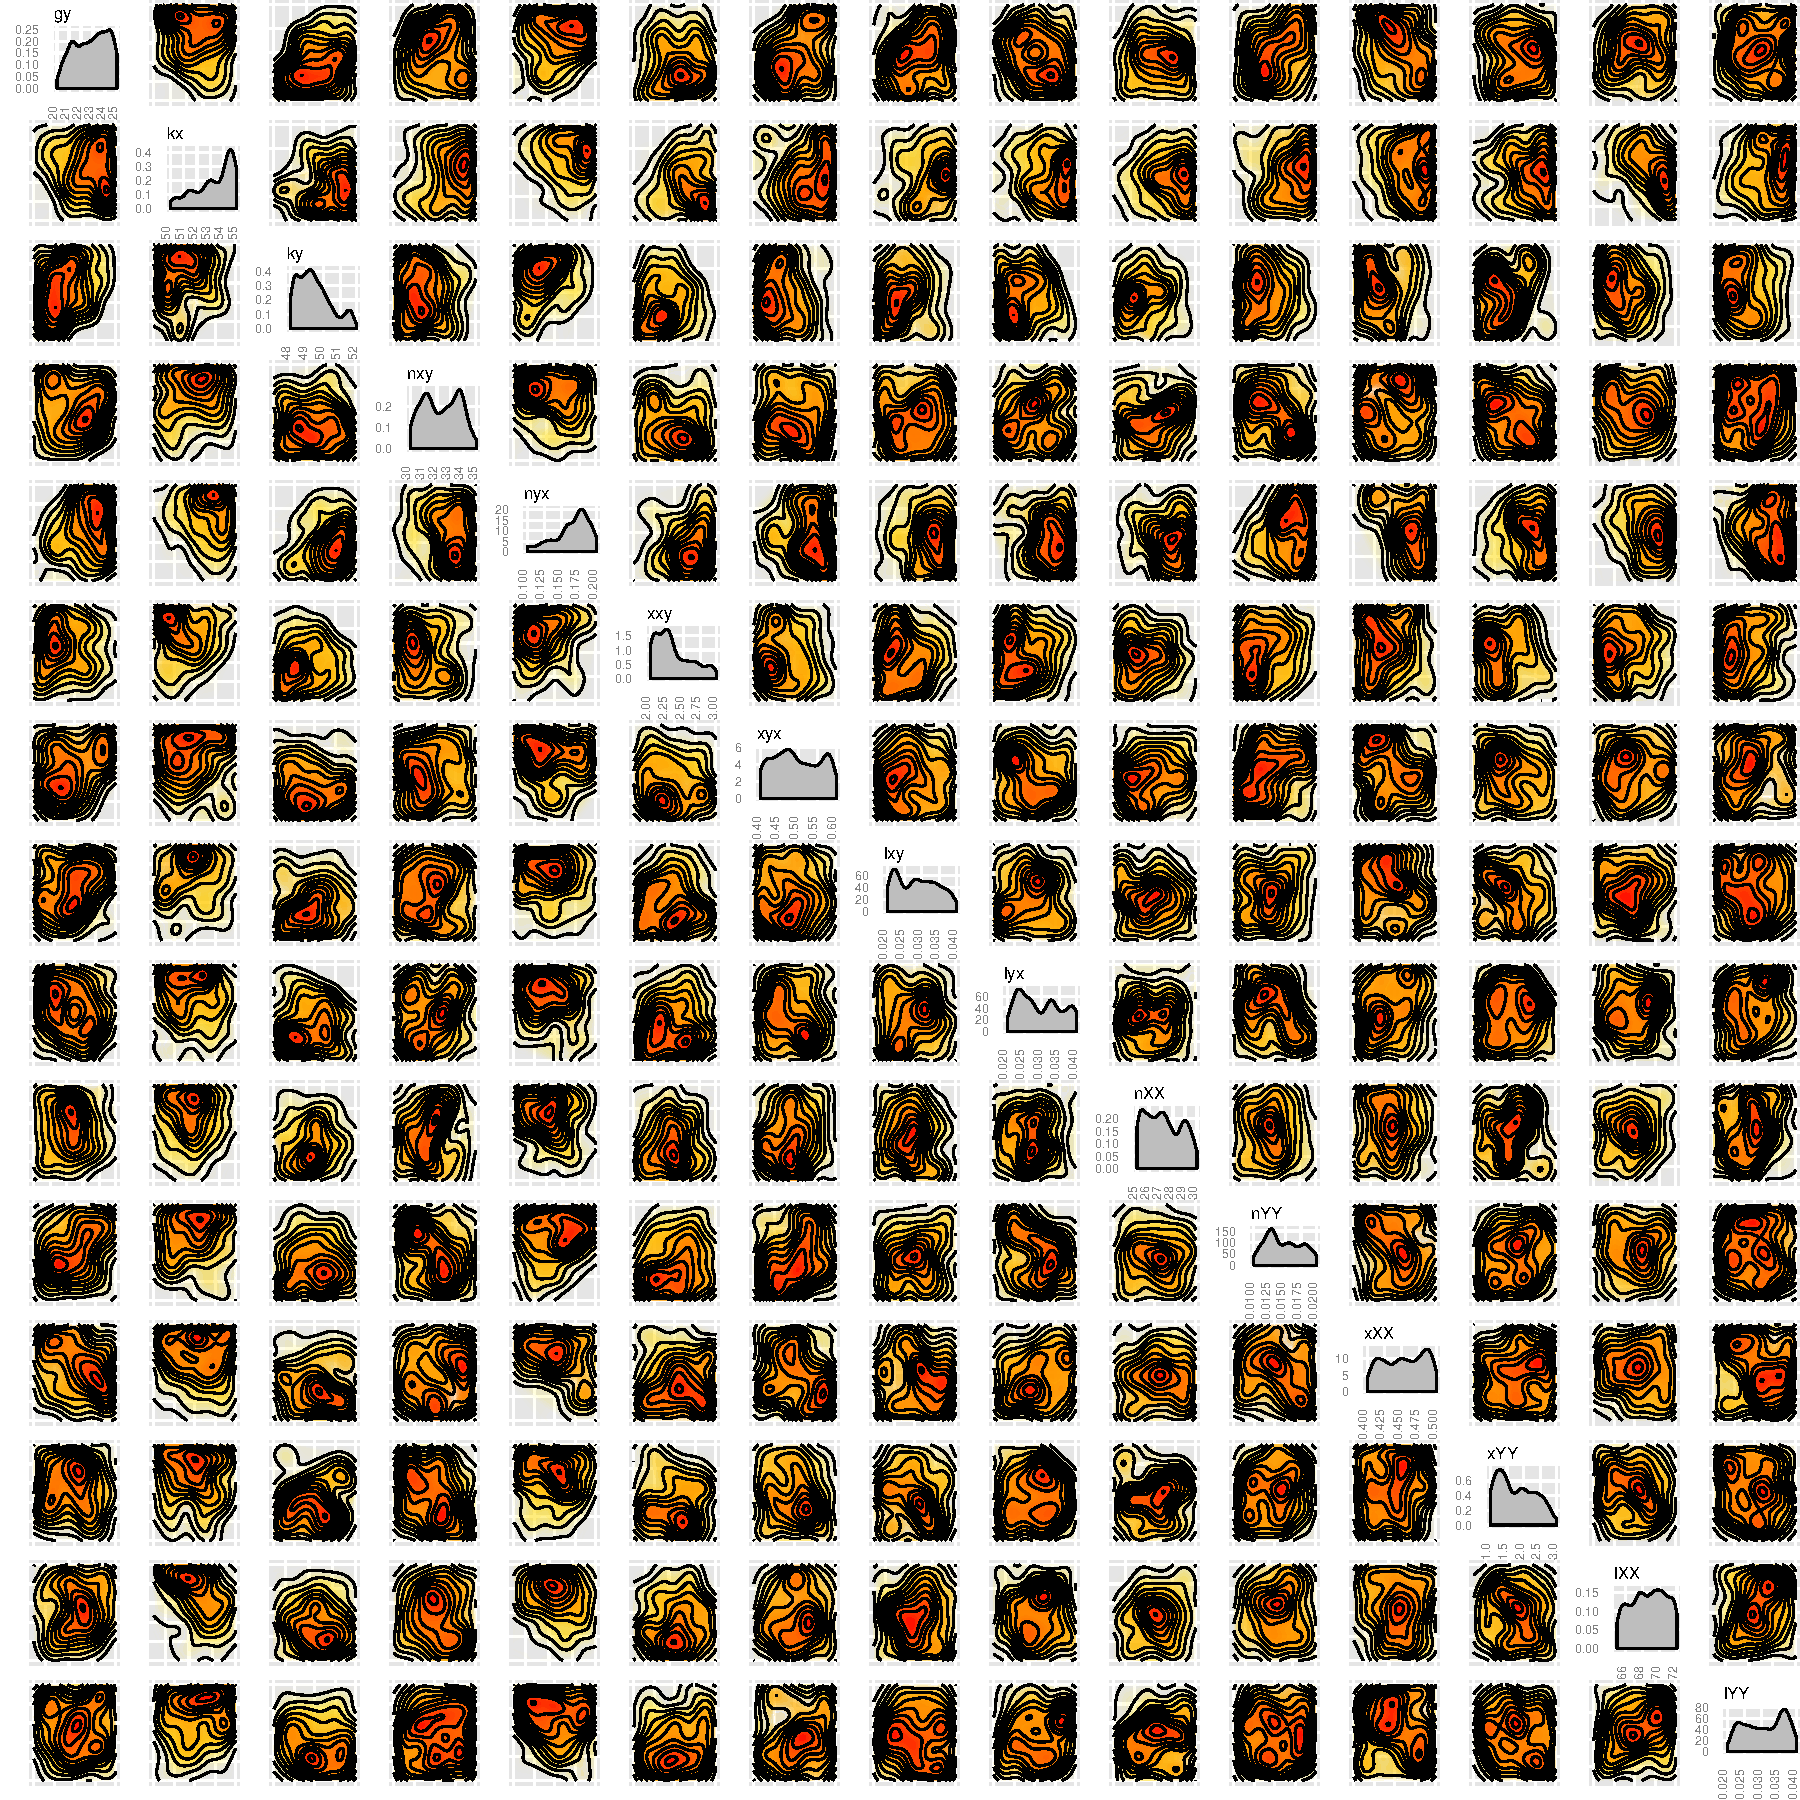
\includegraphics[scale=0.7]{chapterModelling/images/Gardner/posterior.pdf}
\caption[The posterior distribution of the bistable Gardner toggle switch]{The posterior distribution of the bistable Gardner toggle switch. The parameters $a_1$, $a_2$ represent to the effective synthesis rate of repressors 1 and 2 respectively. Parameters $\beta$, $\gamma$ represent the cooperativity on repressors 1 and 2 respectively. The marginal distributions of each parameter are found on the diagonal and pairwise joint distributions along the sides.}
\label{fig:Gard_post}
\end{figure}


\begin{figure}[t]
\centering
\includegraphics[scale=0.3]{chapterModelling/images/Gardner/phase_plots.png}
\caption{A sample of the phase plots produced from the final population of the Gardner switch.}
\label{fig:det_gard_phase}
\end{figure}

\begin{table}[b]
\centering
\caption{Gardner switch priors}
\label{tab:gard}
\begin{tabular}{cccc|cc}
\multicolumn{4}{c|}{Parameters} & \multicolumn{2}{c}{Species} \\ %\hline
$a_1$   & $\beta$   & $a_2$   & $\gamma$  &   $s_1$      &       $s_2$   \\
0-10    & 0-5       & 0-10    &  0-5      &      0-100   &          0-100   
\end{tabular}
\end{table}

These results agree with the results reported by the original paper~\autocite{Gardner:2000vha} . For this switch to be bistable $a_1$ and $a_2$ must be balanced while $\beta$ and $\gamma$ must both be \textgreater 1, as can be seen in the marginal distributions of $\beta$ and $\gamma$ in Figure~\ref{fig:Gard_post}. The conditions set by the original paper for parameters $a_1$ and $a_2$ are met, as the joint distribution shown in Figure~\ref{fig:Gard_post} matches the bifurcation lines calculated in the original paper. 
This successful test demonstrates that StabilityFinder can be used to find the stability a model is capable of as well as the parameter ranges that can produce that. This allows us to confidently apply the methodology to further models.
%-%-%-%-%-%-%%-%-%-%-%-%-%%-%-%-%-%-%-%

\subsubsection{Comparing the deterministic and stochastic cases} 
    
There are two main ways of modelling a system, deterministically and stochastically. Deterministic modelling utilises ordinary differential equations (ODE) and models the concentrations of the species (proteins or other molecules) by time-dependent variables~\autocite{deJong:2002ft}. Rate equations are used to model gene regulation where the rate of production of a species is a function of the concentrations of the other species~\autocite{deJong:2002ft}. When modelling deterministically the model is viewed as a system which, with sufficient knowledge of the system, its behaviour is entirely predictable. Nevertheless we are still a long way away from having complete knowledge of a system of interesting size~\autocite{wilkinson:2006}. Deterministic modelling also assumes a homogenous mixture where species concentrations vary continuously and deterministically, assumptions that often are not met \textit{in vivo}. A cell is spatially and temporally separated, due to small molecule numbers and fluctuations in the timing of processes~\autocite{deJong:2002ft}.  
   
In stochastic modelling, species are measured in discrete amounts rather than concentrations and a joint probability distribution is used to express the probability that at time \textit{t} the cell contains a number of molecules of each species~\autocite{deJong:2002ft}. It takes uncertainty into account and is thus often more appropriate for modelling cellular systems, although more computationally intensive. In stochastic systems the Gillespie algorithm is widely used to simulate the time-evolution of the state of the system~\autocite{Warren:2005kea}.

The toggle switch has been modelled both deterministically and stochastically, with the two methods producing different results. Thus here we use StabilityFinder to compare the stabilities that the model is capable of, under the different simulation types. By using the same framework, and the same prior distributions for the models, one can directly compare the posterior distributions produced by the deterministic and the stochastic case, and uncover the effects that are due to the stochasticity of the system. This is relevant in a a biological model in which small molecule numbers and external noise are not negligible. Using StabilityFinder and using the same priors for the two models (Table~\ref{tab:gard_det_stoch}), we calculated the posterior for each both bistable models. The results are shown in Figure~\ref{fig:Gard_summary}. The prior ranges used are much wider than in the test case in order to allow more flexibility in both models and have a greater range over which to compare the models. 


\begin{table}[h]
\centering
\caption{Gardner switch priors in the deterministic and stochastic cases}
\label{tab:gard_det_stoch}
\begin{tabular}{cccc|cc}
\multicolumn{4}{c|}{Parameters} & \multicolumn{2}{c}{Species} \\ %\hline
$a_1$   & $\beta$   & $a_2$   & $\gamma$  &   $s_1$      &       $s_2$   \\
0-60    & 0-5       & 0-60    &  0-5      &      0-100   &          0-100   
\end{tabular}
\end{table}

\begin{figure}[p]
\centering
\includegraphics[scale=0.45]{chapterModelling/images/Gardner/summary.png}
\caption[The stochastic and deterministic cases of the Gardner toggle switch]{The Gardner toggle switch is modelled stochastically and deterministically. The model is shown graphically and mathematically in (A), The posterior and phase space of the deterministic model is shown in (B) and of the stochastic case in (C).}
\label{fig:Gard_summary}
\end{figure}


%\begin{figure}[p]
%\centering
%\includegraphics[scale=0.5]{chapterModelling/images/Gardner/wide_var/posterior_deter_high_mean.pdf}
%\caption{The posterior distribution of the deterministic model of the Gardner toggle switch.}
%\label{fig:Gard_post_det_high}
%\end{figure}
%
%\begin{figure}[p]
%\centering
%\includegraphics[scale=0.5]{chapterModelling/images/Gardner/wide_var/posterior_stch_high_mean.pdf}
%\caption{The posterior distribution of the stochastic model of the Gardner toggle switch.}
%\label{fig:Gard_post_stch}
%\end{figure}
\clearpage
As can be seen in the above results, stochasticity has a big effect on the posterior. Firstly, a greater parameter range can produce a bistable behaviour when stochastic effects are taken into account. The condition set by T.~S Gardner~\autocite{Gardner:2000vha} for the values of $a_1$ and $a_2$ to be balanced holds in both the deterministic and stochastic cases but in the stochastic case this is met by a wider range of values. The second conditions of $\beta$, $\gamma$ \textgreater 1 also needs to be met in the stochastic case. The posterior of the deterministic model shown in Figure~\ref{fig:Gard_summary}B, parameters $a_1$ and $a_2$ also have an upper limit of values they can take and still create a bistable switch. In order to test this result, we find the roots of the system for large values of  $a_1$ and $a_2$ in order to see if three roots are still found, two stable and one unstable. The results as shown in Figure indicate that the system is still bistable for increasing values of $a_1$ and $a_2$. This suggests that the upper limit found with StabilityFinder is an artefact of the variance limit imposed on the system. In order to find the steady states we impose an accepted distance from a given total variance for each model. When the two clusters of steady state values are too far removed, this increases total variance of the system and would consequently be rejected in StabilityFinder.

\begin{figure}[h]
\centering
\includegraphics[scale=0.6]{chapterModelling/images/Gardner/gardner_solve_roots_a1a2_big.pdf}
\caption[Solving the Gardner toggle switch.]{Solving the Gardner toggle switch. The parameters values used are:  $a_1$, $a_2$ = 100 and $\beta$, $\gamma$ = 2. The system has three roots, of which one was found to be unstable and the other two stable. This result disagrees with that found in StabilityFinder, that $a_1$ and $a_2$ have an upper limit of 30.}
\label{fig:Gard_robst}
\end{figure}

 When stochasticity is taken into account, robustness increases significantly as seen in Figure~\ref{fig:Gard_robst}. This indicates that stochasticity increases the ability of the model to withstand fluctuations in parameter values and still produce the desired bistability. A deterministic model cannot predict this increased robustness.
 
\begin{figure}[h]
\centering
\includegraphics[scale=0.6]{chapterModelling/images/Gardner/wide_var/robustness_comparison.pdf}
\caption{Comparing the robustness of the deterministic and stochastic Gardner switch models}
\label{fig:Gard_robst}
\end{figure}



In order to check if this increase in robustness is caused by the different clustering methods used in the stochastic and deterministic cases, we tested the deterministic case by running the exact same model but using the clustering algorithm used in the stochastic case. Then we compared the robustness using the method outlined above. These results are shown in Figure~\ref{fig:Gard_det_stoch_kmeans}

\begin{figure}[h]
\centering
\includegraphics[scale=0.5]{chapterModelling/images/Gardner/robustness_comparison_gard_stoch_determ_kmeans.pdf}
\caption{The effect of the clustering methods on robustness measurements}
\label{fig:Gard_det_stoch_kmeans}
\end{figure}

This indicates that the clustering methods used have a big effect on the robustness measured. The increase in robustness seen in Figure~\ref{fig:Gard_robst} could be a bias of the clustering algorithms.
\clearpage

\section{Lu toggle switch models}
 
\subsection{Classical model}
\subsection{Single positive autoregulation}
\subsection{Double positive autoregulation}
\subsection{Extracting the design principles of a tristable switch}

\section{Mass Action switches}
\subsection{Deterministic case}
\subsubsection{Symmetric switch}
\subsubsection{Asymmetric switch}
\subsubsection{Including transcription and translation}
\subsection{Stochastic case}
\subsubsection{Bistable} 
\subsubsection{Tristable}
\subsubsection{Extracting the design principles of a tristable switch}

\section{Discussion}

Here we presented a methodology, StabilityChecker, which can identify the region of parameter space that can produce the stability of choice. We demonstrated its use on some known models and extracted stability and robustness information from them. We compared the stability profile of the Gardner toggle switch when modelled deterministically and stochastically in order to uncover the differences that arise from the addition of noise in the modelling. We found that the stochastic model showed increased robustness to noise.

We then applied StabilityChecker to the Lu switches in order to uncover the design principles that make a switch bistable versus tristable. We found that the gene expression parameters were critical for making a tristable switch bistable. This would be in agreement with the dynamics of a tristable switch, in which the third steady state occurs when there is a deadlock situation between the two proteins. When there are small numbers of both proteins involved, one represses the production of the other resulting in both promoters being repressed \autocite{Ma:2012dt}. Given our result we can extrapolate that a higher rate of protein production eliminates the possibility of this deadlock situation happening. Once a promoter is free to produce protein it will produce it in a fast enough rate so that that protein dominates the system and represses the antagonizing promoter before it has the chance to repress it. This dynamic would explain the fact that when all the priors remained the same but gene expression was increased by an order of magnitude, the tristable switch became bistable. 

We also applied StabilityChecker to a synthetic biology design problem. We used two models of the switch, one simple model consisting of two mutually repressive transcription factors and a model with added double positive auto-regulation. Comparing the two models, both capable of bistable behaviour, using StabilityChecker we found that the model with added double positive feedback loops is more robust to parameter fluctuations. This makes it a better candidate for building new synthetic devices based on the toggle switch design. We identified the parameter region within which this models are bistable, information that is important when building such a device in the lab. In the future, by selecting the system components accordingly, the parameter values can be adjusted \textit{in vivo}. For example, the parameter value corresponding to the translation initiation rate can be chosen by selecting the appropriate RBS sequence which given a nucleotide sequence will produce the desired rate \autocite{Holtz:2010bm}, a method developed by Salis \autocite{Salis:2009gk}. Another method to tweak the parameter values \textit{in vivo} is to select the promoter to have the strength corresponding to the levels of gene expression and repression desired. Activity of each promoter can be measured and standardised \autocite{Kelly:2009bj} making this process possible. For a system requiring more than one promoter, these can be efficiently selected from a promoter library using a genetic algorithm created by \textcite{Wu:2011bq}. These standardised interchangeable components with known sequence and activity are what synthetic biology classes as BioBricks \autocite{Kelly:2009bj,Canton:2008fv}. These can be selected and used to construct a desired system and replicate the parameter values found using StabilityChecker.

The methodology we presented here can be applied to a variety of problems as demonstrated. It can be applied to any problem of finding the parameter values that can produce a desired stability between two species. It can be used to design new systems of desired stability and help identify the appropriate parts to use by identifying the rates within which these parts need to operate. It can also be used to examine existing systems and give an insight on the underlying mechanisms that allow for the given stability to occur. 




%% Chapter-5 Designing new switches ---------------------------%%
\mainmatter*
\chapter{Designing new switches}
\section{Circuit overview}

\section{Parts}


%% Chapter-6 Conclusions --------------------------------------%%
\mainmatter*
\chapter{Conclusions}

\printbibliography

%% --------------------------------------------------------------
%% APPENDIX
%% --------------------------------------------------------------
\appendix*
\chapter{Appendix}

\section{Clustering algorithms}

\subsection{Deterministic case}
\begin{algorithm}
  \caption{Clustering the steady state deterministic simulation results}
 \begin{algorithmic}[1]
    \Statex
      
      \For{each data point}
      	\If{first point}
      		\State Make first cluster
      		\State cluster counter = 1
      	\Else
      		\For{each cluster}
      			\If{cluster within cluster means $\pm$ delta}      			
      					\State Add to existing cluster \\
      					\State Update means of clusters
      			\EndIf
      			\If{reached\_end and not assigned to cluster}
      				\State cluster counter +=  1
      				\State Add new cluster

      			\EndIf
      		\EndFor
      	\EndIf
	
      \EndFor

        
  \end{algorithmic}
\end{algorithm}

\subsection{Stochastic case}
\subsubsection{Gap statistic}

\begin{algorithm}
\caption{Choosing the optimal number of clusters}
 \begin{algorithmic}[1]
    \Statex
    
    \Function{Wk}{$clusters, cluster\_centres$}
    	\For{each cluster}
    		\For{each point in cluster}
    			\State $a = $ matrix norm $(cluster\_centre - point)$    			
    		\EndFor
    		\State $dk = \sum((a)^2 )\times (2 \times $ number of points in cluster)
    	\EndFor
    	\State $wk = \frac{ \sum(dk)}{2 \times (number of points in cluster)} $
    	\State \Return $wk$
    \EndFunction
    \Statex  
    \Function{bounding\_box}{$data$}
    	\State $xmin, xmax = $ min and max of x axis in data
    	\State $ymin, ymax = $ min and max of y axis in data
    	\State \Return $((xmin, xmax), (ymin, ymax)) $
    \EndFunction
    
    \Statex
    \Function{Gap\_statistic}{$data, cutoff$}
    	\State $(xmin, xmax), (ymin, ymax)$ = \Call{bounding\_box}{$data$}
    	 	\State $ks = [1,2,3,4]$
    	\For{$k$ in $ks$}
   			\State $cluster_centres, clusters = $ \Call{K\-means}{$data, k, cutoff$}
   			\State $Wk = \log($\Call{Wk}{$clusters, cluster_centres$}$)$
   			
   			\State Create references datasets:
   			\For{$i in range(10)$}
   				\For{$n in range ($length of data$)$}
   					\State $Xb = $ random value between $xmin, xmax$ and $ymin, ymax$
   				\EndFor
				\State $cluster_centres, clusters = $ \Call{K\-means}{$data, k, cut-off$}
  				\State $BWk = \log($\Call{Wk}{$clusters, cluster_centres$}$)$
   			\EndFor   
   			\State $Wkb = \frac{\sum(BWk)}{10} $	
   			\State $sk = \sqrt{\sum(\frac{(BWk - Wkb)^2}{10})}$	
   				
    	\EndFor
    	\State $sk = sk \times \sqrt{1=\frac{1}{B}}$
    	\State \Return $ks, Wk, Wkb, sk, data_centres, clusters$
    \EndFunction

    \Statex
	\Function{Distance}{data, cutoff}
		    \State $ks, logWks, logWkbs, sk, clusters\_means, clusts = $\Call{gap\_statistic}{$data, cut-off$}
		    \For{$i$ in range $ks$}
		    	\State $gaps = logWks - logWkbs$
		    \EndFor
		    \Let{$cluster\_counter$}{$0$}
		    \For{$i$ in range $gaps$}
		    	\State $cluster\_counter += 1$ 
		    	\If{end}
		    		no clustering
		    	\EndIf
		    	\If{$gaps[i] \geq (gaps[i+1]-sk[i+1])$}
		    		\State Break 
		    	\EndIf
		    \EndFor
	\State \Return $cluster\_counter, clusters\_means[cluster_counter]$
	\EndFunction


  \end{algorithmic}
\end{algorithm}

\subsubsection{K-means clustering}
\newpage
\begin{algorithm}
\caption{Clustering stochastic case}
 \begin{algorithmic}[1]
    \Statex
    
    \Function{K\-means clustering}{$data, k, cutoff$}
    	\Statex
    	\Function{Update\_centres}{$old\_centres, values$}
    		\State $centre\_coords = $ mean for each dimension
    		\State $shift = $\Call{getDistance}{$centre\_coords, old\_centres$}
    		\State \Return $shift, centre\_coords$
    	\EndFunction
    
    	\Statex
    	\Function{getDistance}{$a, b$}
    		\State $dist = \sqrt{(a[x] - b[x])^2+(a[y] - b[y])^2}$
    		\State \Return $dist$
    	\EndFunction
      
      	\Statex
      	\While{True}
      		\For{each point in data}
      			\For{each cluster}
      				\State $dist = $\Call{getDistance}{point, cluster centre}
      			\EndFor
      			\State Find cluster with minimum distance
      			\State Repopulate clusters
      		\EndFor
      		
      		\Let{biggest\_shift}{0}
      		\For{as many times as there are clusters}
      			\State $shift$, cluster centres $=$ \Call{Update\_centres}{$old\_centres, clusters$}
      			\State $biggest\_shift = $ max between $shift, biggest\_shift$
      			
      		\EndFor
      		\If{$biggest\_shift \leq cutoff$}
      			\State break
      		\EndIf
      	\EndWhile
      \State \Return $cluster\_centres, clusters$
    \EndFunction

  \end{algorithmic}
\end{algorithm}


\end{document}